\documentclass[journal, letterpaper]{IEEEtran}

\usepackage{graphicx}
\usepackage[english]{babel}
\usepackage[square,numbers,super]{natbib}
\bibliographystyle{abbrvnat}

\usepackage{ mathrsfs }
\usepackage{braket}
\usepackage{url}        
\usepackage{amsmath}   
\usepackage{amssymb}
\usepackage{textgreek}	% Greek to me, dawg
\usepackage{listings}
\usepackage{csvsimple}
\usepackage{longtable}
\usepackage{siunitx}
\begin{document}
    
	\title{% 
                Information Theory Project
                %\large Literature review of the 
            }

	\author{Roberto Scardia, Gabriele Lecce}
	\maketitle

\section{Introduction}
In this literature review, we will lay out the necessary quantum mechanics and quantum information concepts needed to understand the meaning and consequences of the Holevo's bound in quantum information theory. We will show that classical information theory is a particular case of quantum information theory, and in the final part we will discuss some applications of quantum mechanics in the field of optical communications. In particular, we will focus on the adverse impact of non-ideal effects on the information rate of continuous variable quantum key distribution protocols.
    
\section{Quantum mechanics}

Reasonably, a treatise on quantum mechanics should start with the definition of quantum states: historically, they evolved from the classical concept of "state" for a dynamic system. In classical physics, to describe the evolution of a dynamic system, it is not sufficient to know only the physical law that governs that particular system. It is also required to use the information given by the values of the state variables that describe the system, and, in general, it is possible to organize these values inside a "state vector". 
In the same way, a "quantum state" is the mathematical entity that embeds the information needed to describe the evolution of a quantum system.\\ 
Quantum mechanics is the mathematical theory that describes the preparation, evolution, and measurement of a quantum system. By itself, quantum mechanics does not describe the physical law that a particular quantum system must obey, but it is useful as a framework to develop the mathematical foundation of other physical theories. Indeed, we will not reference any specific physical implementation while talking about quantum states, qubits, and measurements, but we will stop at the general mathematical description.
The most useful mathematical representation of a quantum state for quantum information is the vector representation: in the same way classical states can be organized in vectors, the quantum states are thought to be components of a Hilbert space equipped with a scalar product. 
A Hilbert space is the generalization of the classical Euclidean vector space to possibly infinite dimension spaces where the classical ideas of (but not limited to) scalar product, distance, Pythagorean theorem, and Cauchy-Schwarz inequality still hold. The need for infinite-dimensional Hilbert space in quantum mechanics presents itself in the case, for example, of the more known wave representation of quantum states; however, it is not strictly needed in our review for it will be shown that quantum information theory limits its scope to systems described by two-dimensional Hilbert space. 
In the vector representation, an isolated quantum state is a unidimensional subspace of a Hilbert space $\mathscr{H}$: every vector $\ket{\psi} \in \mathscr{H}$ represents a different state apart from a complex constant $\lambda$, and every vector belonging to the same "line" or "ray" represents the same (isolated) quantum state. 
This kind of isolated state (i.e., not considered in an ensemble with other quantum states) is called a pure state, and, in general, it is regarded as its representative vector an element of its subspace with norm one, that is, $\bra{\psi}\ket{\psi} = 1$. Note that multiple such normalized vectors exist and are distinguished by a pure phase factor $e^{i\phi}$. Hence we can affirm that a pure quantum state, in reality, is a member of a projective Hilbert space, defined from a Hilbert space $H$ as the set of the equivalence classes $[v]$ of $ v \neq 0 \in \mathscr{H}$ with the equivalence relationship $\sim$ such that \( \forall v, w \in \mathscr{H} \: v \sim w \iff \exists\lambda \in \mathbb{C}\:|\: w = \lambda v \).
What we described in the previous section is the first postulate of quantum mechanics: \\ \\
\begin{minipage}{\linewidth}
    \textbf{Postulate 1}: Associated to any isolated physical system is a complex vector space with inner product (that is, a Hilbert space) known as the state space of the system. The system is fully described by its state vector, which is a unit vector in the state space of the system. \cite{chuang}
\end{minipage}\\ \\

From the theory of linear algebra, it is known that every element belonging to a vector (Hilbert) space can be expressed as a linear combination of the basis of the same space.
\[\mathscr{H} = \mathscr{L} \{B_{\mathscr{H}}\}\]
In quantum mechanics, this property of Hilbert spaces is called "superposition": each state can be expressed as the superposition of different states multiplied by a complex constant.\\
We said earlier that quantum information limits its scope to two-dimensional state space: the elements of such spaces are called qubits (from the portmanteau of quantum bits). Typically the canonical basis of a qubits space is denoted as \[\ket{0} = \begin{bmatrix}
           1 \\
           0 \\
           \end{bmatrix},
\ket{1} =  \begin{bmatrix}
           0 \\
           1 \\
           \end{bmatrix}\] 
but others are known such as the computational basis \[\ket{+} = (\ket{0} - \ket{1})\frac{1}{\sqrt{2}} \]
\[\ket{-} = (\ket{0} + \ket{1})\frac{1}{\sqrt{2}} \]

In general, a pure quantum state is nearly impossible to be physically realized and we have to resort to a probabilistic description of our quantum system. These uncertain states are called "mixed states" and arise not only in the preparation of real quantum systems but also in the case of entangled states.\\ 
Such description can be obtained by modeling it as an ensemble of pure quantum states $\psi_{i}$ with a priori probabilities $p_i$ using the concept of density operator $\rho$: 
 \[\rho = \sum_{i}p_i\ket{\psi_i}\bra{\psi_{i}}\]
The density operator can also be defined for a pure state $\psi$ as: 
\[\rho_\psi = \ket{\psi}\bra{\psi}\]
 
That can be generalized in the case that our quantum system is in a mixed state:
\[\rho = \sum_i p_i \rho_i\]
Where $\rho_i$ is the density operator of the pure states that compose the ensemble. It's easy to verify that $\rho$ is always positive and its trace is equal to one. 

Mixed states are not to be confused with the superposition of states: superposition results from the linearity of the operator that governs the quantum processes and no probability is involved until the measurement of such states occurs.

We said earlier that quantum mechanics does not describe the physical laws that govern the physical systems taken into consideration, but gives an important description in the form of its second postulate:\\

\begin{minipage}{0.96\linewidth}
\textbf{Postulate 2}: The evolution of a closed quantum system is described by a unitary
    transformation. That is, the state $\ket{\psi}$ of the system at time $t_1$ is related to the state $\ket{\psi}'$
    of the system at time $t_2$ by a unitary operator U which depends only on the times $t_1$ and $t_2$ \cite{chuang}
\end{minipage} \\ \\

Note that the postulate does not state anything about U other than it being a unitary operator. A unitary operator $U$ is a linear operator defined on a Hilbert space such that $UU^\dagger = U^\dagger U = I$. Note that U is a linear operator and this comes in handy when considering the superposition principle: having decided a basis, each operator can be defined as the matrix of the column images of the basis elements.\\
We will not dwell on every mathematical implication of this definition but it will be useful later to cite the alternative postulation involving the \textit{Schr{\"o}dinger's equation}:\\ \\

\begin{minipage}{0.96\linewidth}
\textbf{Postulate 2'}: The time evolution of the state of a closed quantum system is described by the \textit{Schr{\"o}dinger's equation}, \[i\hbar\frac{d\ket{\psi}}{dt} = H\ket{\psi}\] In this equation, $\hbar$ is a physical constant known as Planck’s constant whose value must be experimentally determined. The exact value is not important to us. In practice, it is common to absorb the factor $\hbar$ into $H$, effectively setting $\hbar$ = 1. $H$ is a fixed Hermitian operator known as the Hamiltonian of the closed system. \cite{chuang}
\end{minipage} \\ \\
The Hamiltonian is the operator related to the total energy of the quantum system taken into consideration and its expression is dependent on the physical description of the system; i.e. quantum mechanics still does not describe the physical law of the system but just their properties.

What our discussion on quantum mechanics lacks at this point is a description of what happens during the measurement process: when a quantum state is measured, the quantum system has to interact with the measurement apparatus so it cannot be considered a closed quantum system and the second postulate cannot be considered valid. In the same way that QM doesn't describe the laws involved with the evolution of the system, it does not prescribe a particular apparatus or practical procedure to carry out a quantum measure but lays out the mathematical foundation to describe the results.\\
The third and last postulate of QM states the following:\\ \\

\begin{minipage}{0.96\linewidth}
\textbf{Postulate 3}:  Quantum measurements are described by a collection {$M_m$} of measurement operators. These are operators acting on the state space of the system being measured. The index $m$ refers to the measurement outcomes that may occur in the experiment. If the state of the quantum system is $\ket{\psi}$ immediately before the measurement then the probability that result $m$ occurs is given by
\[p(m) = \bra{\psi}M^\dagger_m M_m\ket{\psi}\]
and the state of the system after the measurement is
\[\frac{M_m\ket{\psi}}{\bra{\psi}M^\dagger_m M_m \ket{\psi}}\]
The measurement operators satisfy the completeness equation,
\[\sum_m M^\dagger_m M_m = I\]
The completeness equation expresses the fact that probabilities sum to one:
\[ \sum_m p(m) = \sum_m \bra{\psi}M^\dagger_m M_m\ket{\psi}=1\cite{chuang}\]
\end{minipage} \\ \\
The states here are considered to have norm equal to one.
A quantum measure involves necessarily a probabilistic description: while in classical physics we need a statistical description (being classical or Bayesian) to account for noise and measurement error, in QM the result of the measurement operation is intrinsically probabilistic. 
For example, a valid example of measurement operator collection on qubits is the set composed by the density operator of the canonical basis, \(M_0 = \ket{0}\bra{0}\), \(M_1 = \ket{1}\bra{1}\). If we consider a state $\psi = a\ket{0} + b\ket{1}$ the probability of measuring the state 0 or 1 is:
\[p(0/1) = \bra{\psi}M_{0/1}^\dagger M_{0/1} \ket{\psi} = \bra{\psi} M_{0/1} \ket{\psi} = |a/b|^2\] 
where the hermiticity property of the density operator $(M_{0/1} =M_{0/1}^\dagger, M_{0/1}^2=M_{0/1}$ is used. 
In this specific example, we choose to use the density operator of two orthogonal states ($\bra{0}\ket{1} = 0$, by definition of canonical basis) and if the state $\psi$ were equal to 0 or 1 we would have been able to measure 0 or 1 with probability 1 respectively. However, this is only true for states that are orthogonal, and, in general, for two states that are not orthogonal it does not exist a measurement set with this property. For this reason, two states that are not orthogonal are called \textit{non-distinguishable states}.\\
In general, the operators in the measurement set do not have to be unitary. In case they possess this property (i.e. the second postulate is respected during the measurement) and are orthogonal ($M_mM_n = 0 \; for\; m \neq n$) we are in the special case of \textit{projective measurement}. In projective measurement, an operator $M$ called \textit{observable} is defined with spectral decomposition \[M = \sum_m mP_m\] where $m$ is one of its eigenvalue and $P_m$ the orthogonal projectors over its eigenspaces; those compose the measurement set. The previous example can be understood as a case of projective measurement and the same simplifications for calculating the probability distribution can be applied:
\[ p(m) = \bra{\psi}P_m\ket{\psi}\] The resulting state after a projective measurement is \( \frac{P_m\ket{\psi}}{\sqrt{p(m)}}\) i.e. one of the states described by the eigenspaces of $M$.\\   
Another special case of the third postulate that is thoroughly used in quantum information is the Positive Operator-Value Measure: instead of singularly choosing the measurement operators $M_m$ such that they respect the completeness equation as a measurement set whatever choice of $E_m$ such that \(\sum_m E_m = I\). This formalism is useful whenever after the measure there is no interest in the state of the system or the measurement is not repeatable. By definition, projective measurement describes a repeatable procedure: after obtaining the state $\ket{\phi_m}$ as the result of the measure by repeating the measurement with the same set we re-obtain $\ket{\phi_m}$ with probability one. In quantum information we are often only interested in the statistics of the measure and not in the evolution of the system and the utility of this formalism will be shown in the following paragraphs.
\\ 
\\
A quantum phenomenon that plays an important role in both quantum information theory and quantum cryptography is the no-cloning theorem. Suppose that we have a device that can duplicate quantum states: 
if we want to copy a pure state $\ket{\psi}$ in a blank state $\ket{X}$ we have to apply a unitary operator on the system: 
\[U\ket{\psi}\ket{X} = \ket{\psi}\ket{\psi} \]
And this is true for all the orthogonal $\ket{\psi_i}$ forming a space vector. However, it's not possible to duplicate a non-orthogonal state \cite{clone} e.g. $\ket{\psi} = \frac{1}{\sqrt{2}}(\ket{0}+\ket{1})$: 
\[U\frac{1}{\sqrt{2}}(\ket{0}+\ket{1})\ket{X} = U\frac{1}{\sqrt{2}}(\ket{0}\ket{X}) + U\frac{1}{\sqrt{2}}(\ket{1}\ket{X}) = \] \[=\frac{1}{\sqrt{2}}\ket{0}\ket{0} +\frac{1}{\sqrt{2}}\ket{1}\ket{1}\]
That is different from what we expected: 
\[ \frac{1}{\sqrt{2}}{(\ket{0}+\ket{1})\frac{1}{\sqrt{2}}}(\ket{0}+\ket{1}) \neq  \frac{1}{\sqrt{2}}\ket{0}\ket{0} +\frac{1}{\sqrt{2}}\ket{1}\ket{1}\]
\section{Quantum information}
In “classical” information theory Shannon’s entropy is defined as the measure of information of a memory-less stationary source, for which we know the probability $P(X)$ of a set of symbols \{X\}: \[H(X) = - \sum_{X} P(X)\log_2P(X)\]
To describe a set of quantum states \{$\psi$\}, probability distributions are replaced by density operators. The natural extension of the Shannon’s entropy is the Von Neumann entropy, defined as:
\[S(\rho) = -tr(\rho \log\rho) = -\sum_{\psi} \lambda_{\psi}\log\lambda_{\psi} \]
Where $\lambda_{\psi}$ are the eigenvalues of the density operator $\rho$. 
We can easily verify that if the states of the alphabet are orthogonal (e.g. $\{X\} = \{\ket{0},\ket{1}\}$), the Von Neumann entropy coincides with Shannon's entropy: 
\[\rho = p\ket{0}\bra{0} + (1-p)\ket{1}\bra{1} = \begin{bmatrix}
    p & 0 \\
    0 & 1-p
\end{bmatrix}\]
\[\Rightarrow S(\rho) = -p\log_2p -(1-p)\log_2(1-p) = \log_2\frac{(1-p)^{p-1}}{p^p} \]
That coincides with Shannon's entropy of a binary source. Suppose the dimension d of the space vector $C^d$ can be considered as the number of symbols in a classical alphabet. In that case, the Von Neumann entropy is upper bounded by: \[S(\rho) \le log_2(d) \] And in general, for an ensemble of non-orthogonal pure quantum states (in this case $\rho$ is not hermitian) we have: \[S(\rho) \le H(X)\] It is possible to verify that the single pure state $i$ of the ensemble has the property $S(\rho_i) = 0$. In the most general case, when an ensemble of mixed states describes our system, we have the following upper bound: 
\[S(\rho) \le \sum_{i}p_iS(\rho_i) + H(X)\] that is held with equality only when the states $\rho_i$ have orthogonal support. If we rewrite the last expressions as follows: 
\[S(\rho) - \sum_{i}p_iS(\rho_i) \le  H(X)\]
We can identify a quantity: \[\chi(\rho_i) = S(\rho) - \sum_{i}p_iS(\rho_i)\] that is the Holevo information of our ensemble. This quantity can be regarded as a generalization of the Von Neumann entropy when we send messages constructed from an alphabet of non-orthogonal mixed states. It will play an important role when we will describe the Holevo's bound.
\\
\\
When we use non-orthogonal states, a new “quantum” problem arises. Suppose that our source can only send symbols from an ensemble of two non-orthogonal states e.g. \{$\ket{0}, \frac{\ket{0}+\ket{1}}{\sqrt{2}}$\} and we want to measure them with a set {E} of POVM elements. We can define: \[E_1 = \frac{\sqrt{2}}{1+\sqrt{2}}\ket{1}\bra{1},\] \[E_2 = \frac{\sqrt{2}}{1+\sqrt{2}}\frac{(\ket{0}-\ket{1})(\bra{0}-\bra{1})}{2}\] such that we always have state $\frac{\ket{0}+\ket{1}}{\sqrt{2}}$ when we measure $E_1$ and state $\ket{0}$ when we measure $E_2$. However the set \{$E_1,E_2$\} does not satisfy completeness relation $\sum_mE_m = I$, which is only satisfied by adding a third operator $E_3 = I- E_1-E_2$, that gives no information about the identity of the measured the state: \[\bra{\psi_i}E_3\ket{\psi_i} \neq 0,1 \] That means that if we use non-orthogonal states we don't have perfect reliability. This is the accessible information problem, and can be seen as a direct consequence of the no-cloning theorem. This is never seen in classical information theory, since its symbols are always pure orthogonal states. To quantify how can we know about the accessible information, we can use another classical information theory concept known as mutual information: 
\[I(X,Y) = H(X) - H(X|Y)\]
This is a measurement of the degree of correlation between two random variables, in our case the state measured is Y and the state sent is X. In classical noiseless channels, the mutual information is always equal to the Shannon entropy of the source, since there isn't a problem with accessible information. We expect that in quantum information this inequality holds: \[I(X,Y) \le H(X)\]and it's not satisfied with equality when my quantum system isn't described by orthogonal states. In the next chapter, we wish to connect the Holevo quantity and the mutual information to get more general results.  



\section{Holevo's bound}

The Holevo's bound is one of the most important results in quantum information theory.
Suppose that one actor has prepared a quantum state with density operator $\rho_X$ choosing over $n$ different possible states with probability $p_x \; \; x \in [0,n]$. A second actor has then measured this state with a POVM set $E_y = {E_0, ..., E_y}$ with measure outcome Y. The Holevo's bound states that for such measurement:
\[I(X,Y) \leq S(\rho) - \sum_x p_xS(\rho_x) = \chi\]

where \(\rho = \sum_x p_x \rho_x \) and $\chi$ is the Holevo $\chi$ quantity. 

Using Holevo bound and the results from the previous chapter, we can relate the mutual information of a quantum source described by an alphabet of mixed states with Shannon's entropy of that source: 
\[ I(X,Y) \le \chi(\rho_i)\le H(X)\]
This means that the mutual information is strictly less than $H(X)$ when $\rho_i$ doesn't have orthogonal support, or in other words, when the mixed states of the alphabet are not orthogonal. This is the generalization of what was shown in the previous chapter for the simplified case of a quantum system with an alphabet of non-orthogonal pure states. 
\\
\\
To show the importance of the orthogonality of the mixed states, let's switch for a moment to a 3-dimensional Hilbert space. Suppose we take $\rho_i$ from the ensemble of pure orthogonal states ${X}=\{\ket{0},\ket{1},\ket{2}\}$.  We choose $\rho_1 = q\ket{0}\bra{0} + (1-q)\ket{1}\bra{1}$ and $\rho_2 = p\ket{1}\bra{1}+(1-p)\ket{2}\bra{2}$ to be the mixed states of our system. The density operator of the system is $\rho = \frac{1}{2}\rho_1 + \frac{1}{2}\rho_2$, so the Holevo quantity is upper bounded by the binary entropy: H(X) = 1. When $q=1$ or $p=0$, the mixed states are orthogonal, so we expect the Holevo quantity to be independent of respectively $p$ or $q$. We compute the Von Neumann entropies for this system: 

\[\rho_1 = \begin{bmatrix}
    q & 0 & 0 \\
    0 & 1-q & 0 \\
0 & 0 & 0
\end{bmatrix} \Rightarrow S(\rho_1) = H_2(q);\]
\\
\[\rho_2 = \begin{bmatrix}
    0 & 0 & 0 \\
    0 & p & 0 \\
0 & 0 & 1-p
\end{bmatrix} \Rightarrow S(\rho_2)=H_2(p);\]
\\
\[\rho = \frac{1}{2}\begin{bmatrix}
    q & 0 & 0 \\
    0 & (1-q)+p & 0 \\
0 & 0 & 1-p
\end{bmatrix}\] 
\\
\[ \Rightarrow S(\rho)=-\frac{1}{2}[q\log(\frac{q}{2})+(1-p)\log(\frac{1-p}{2}) +(1-q+p)\log(\frac{1-q+p}{2})]\]
\[= 1+\frac{1}{2}(H_2(p)+H_2(q)+\log\frac{p^p(1-q)^{1-q}}{(1-q+p)^{1-q+p}}) \]
We can finally write the Holevo quantity $\chi$: 
\\
\[\chi(q,p) = S(\rho)-\sum_ip_iS(\rho_i) = 1+\frac{1}{2}\log\frac{p^p(1-q)^{1-q}}{(1-q+p)^{1-q+p}} \]
\[\Rightarrow \chi(q,p) = 1+ G(q,p) \le H(X) = 1\]
And as we expected: \[G(1,p) = G(q,0) = \log_21 = 0 \Rightarrow \chi = 1 = H(X)\]
\begin{figure}[!h]
    \centering
    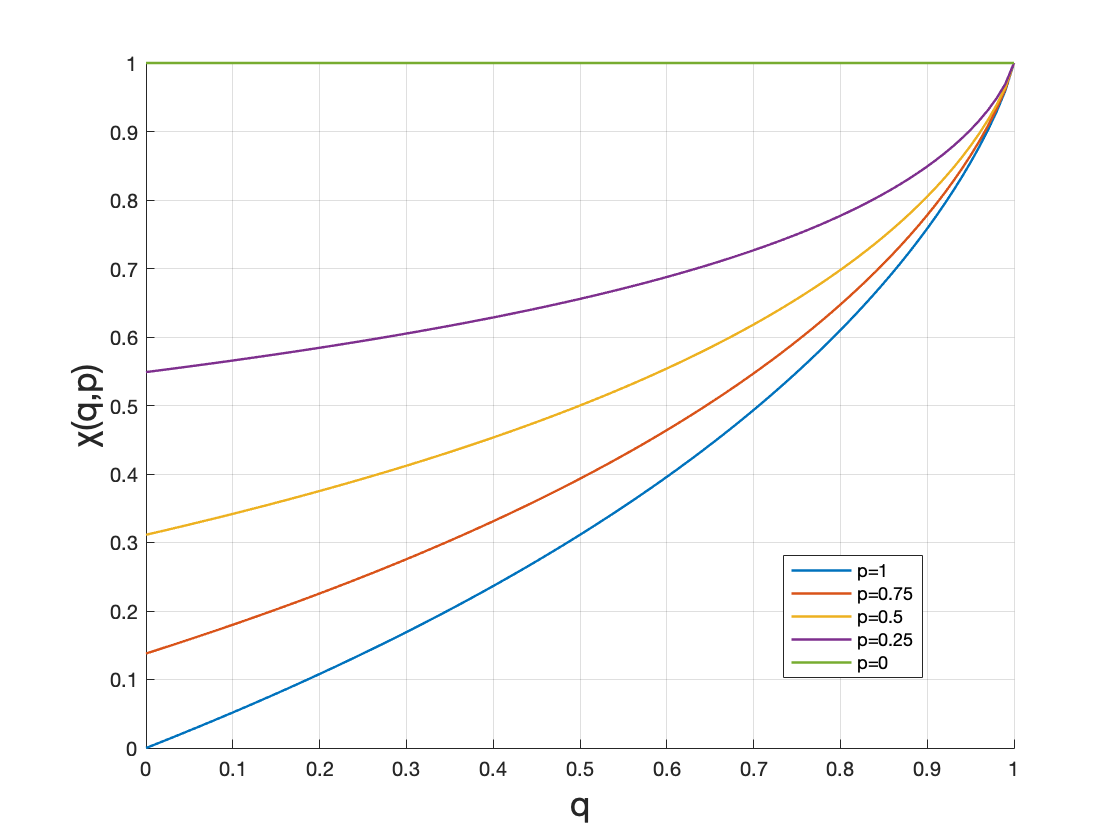
\includegraphics[width=0.5\textwidth]{Images/graficus.png}
        \caption{Holevo quantity $\chi$ as function of q and p.}
     \label{fig:quadtree}
\end{figure} 
\\
If $p$ it's set and we increase $q$, the Holevo quantity increases because the mixed states approach the orthogonality condition. The mutual information of this quantum system is upper bounded by:
\[I(X,Y) \le 1\]
If we choose a proper POVM set and two orthogonal mixed states, we can achieve $I(X,Y) = 1$. Suppose to pick the particular case $\{X\} = \{\frac{1}{2}(\ket{0}+\ket{1}),\ket{2}\}=\{\ket{\psi_1},\ket{\psi_2}\}$, we can calculate the POVM as: 
\[\bra{\psi_1}E_1\ket{\psi_1} = 1 \Rightarrow E_1 = \begin{bmatrix}
    1 & 0 & 0 \\
    0 & 1 & 0 \\
0 & 0 & 0
\end{bmatrix} \]

  \[\bra{\psi_2}E_2\ket{\psi_2} = 1 \Rightarrow E_2 = \begin{bmatrix}
    0 & 0 & 0 \\
    0 & 0 & 0 \\
0 & 0 & 1
\end{bmatrix} \]
Where the completeness relation has been used to maximize the mutual information: 
\[ \sum_mE_m = E_1 + E_2 = I\]
We have found that optimal measurement determined by the ensemble has the property: 
\[p(m) = \delta_{m,x}\]
Where $\delta_{m,x}$ is the Kronecker delta. We can now better define the concept of accessible information as the maximization of the mutual information over all the sets $\{E_m\}$ of possible POVM measurements: 
\[I_{acc} = \max_{\{E_m\}}{I(X,Y)} \]

We have seen that orthogonal states are perfectly distinguishable, however it's not possible to maximize the mutual information in this way when the mixed states are non-orthogonal ($\chi <H(X)$). If we use an alphabet of pure states (to simplify the expression of $\chi$), we expect that: 
\[I(X,Y) \le \chi = S(\rho) < H(X)\]
Furthermore, it's also more complicated to guess what is the optimal POVM measurement.
In some cases we can exploit symmetries, for example, if we take an ensemble of pure states which have a three-fold symmetry e.g.: \\\[\{\psi_i\} =\{\cos(\frac{2\pi}{3}*n)\ket{0}+ \sin(\frac{2\pi}{3}*n)\ket{1}\} = \]\[\{\ket{0},-\frac{1}{2}\ket{0}+\frac{\sqrt{3}}{2}\ket{1},-\frac{1}{2}\ket{0}+-\frac{\sqrt{3}}{2}\ket{1}\}\]
with n=0,1,2 and the same a priori probabilities, it is possible to construct an optimal POVM with the same symmetry, that achieves: \[I_{acc} \simeq 0.58496 < S(\rho) = 1\cite{caltech}\] We could try and group states in a similar way to classical information theory: \[\ket{\psi} = \ket{\psi_i}_1\ket{\psi_i}_2...\ket{\psi_i}_m\]
In this way, we would have $3^m$ possible "codewords". However, it is possible to demonstrate that the accessible information doesn't change. A better strategy is the Peres-Wootters method \cite{peres}: instead of using all the $3^m$ codewords built before, we just use three codewords formed by repeating m times one of the three pure states of the ensemble, e.g. for the first state: 
\[\ket{\psi_1} = \ket{0}_1\ket{0}_2...\ket{0}_m\]
In this way the three new states $\ket{\psi_i}$ are more distinguishable; for the case m = 2 we have an improvement of the Von Neumann entropy: 
\[S(\rho)_{m} = S(\rho)_{2} = 1.5 < H(X) = \log_23 \]
We can say that they are more distinguishable because the inner product with the other states is more orthogonal increasing $m$, in other words:  \[\bra{\psi_i}\ket{\psi_j}_m>\bra{\psi_i}\ket{\psi_j}_{m+1},  i \neq j\]
In fact for the $m=2$ case, we improve the maximum mutual information: 
\[I_{acc, m=2} = 1.36907 >  0.58496 \]
The most fundamental concept that the Peres-Wooters method highlights is that it's better to group qubits to create an alphabet with just the more distinguishable letters. Furthermore, we want to measure these states using a POVM constructed by a procedure called  PGM ("pretty good measurements")\cite{caltech}, which gives the maximization of the mutual information.
\\
\\We can also extend this method to an ensemble of non-orthogonal mixed states, saying that when $m\rightarrow \infty$ the accessible information tends to the Holevo's quantity: 
\[I_{acc,m\rightarrow\infty } \rightarrow \chi(\rho_i) \]
We can say, from what we have shown in this review, that the accessible information plays a role similar to the capacity of a channel in classical information theory: it tells us how many "classical" bits of information can be reliably transmitted over the channel. In order to have a good accessible information, we can maximize the Holevo's quantity by using longer codewords and by choosing the optimal POVM set of the system.


\section{Discrete-Variable QKD}
One of the most important applications of quantum information theory and cryptography is Quantum Key Distribution:
a secret key is exchanged through a quantum communication channel using quantum states, and then it can be used as a one-time pad key in a cryptosystem\cite{magarini}. The BB84 protocol is the first QKD protocol ever proposed, and it was made by Charles H. Bennett and Gilles Brassard in 1984 \cite{bb84,moderncrypto}. It exploits the polarization of photons, a continuous parameter that can be regarded quantistically as the photon spin\cite{spin}, a vector in a 2-dimensional Hilbert space, hence a qubit. In classical communication, channel messages can be secretly monitored by an eavesdropper without the knowledge of the sender or the receiver; in QKD when the qubits are intercepted, the no-cloning theorem assures that they can only be measured by perturbing their state, so the receiver may notice that someone was eavesdropping the channel by receiving unexpected results. At first, without considering eavesdropping, the protocol works as follows: a sender (Alice) prepares with equal probabilities a photon in a rectilinear polarization (state $\ket{0}$ or $\ket{1}$) or in a diagonal polarization (state $\frac{1}{\sqrt{2}}\ket{0}+\frac{1}{\sqrt{2}}\ket{1}$ or $\frac{1}{\sqrt{2}}\ket{0}-\frac{1}{\sqrt{2}}\ket{1}$) and sends it to the receiver (Bob). The different states of a polarization basis encode bit 0 or bit 1. We define as the efficiency of retrieving the secret key the capacity of
the channel, which in the case of fixed source probabilities is just the mutual information.
Our quantum system can be described by the matrix: 
\[\rho = \begin{bmatrix}
    3/4 & 0 \\
    0 & 1/4   
\end{bmatrix}\] 
Which gives $I_{acc} = \chi = 0.3113$ [bits/channel use]. This means that on average we have to use the channel $1/I_{acc} \simeq 3.21$ times to get a bit of the secret key. However, this is not the actual functioning mechanism of QKD. After having received all the qubits, Alice and Bob communicate over an ordinary non-quantum channel to compare the polarization basis used to send and receive the message. This operation is called basis \textit{reconciliation}, and when the same basis is used, Bob can keep the content of the qubit; otherwise, the received bit must be discarded. Following this procedure, the newly generated secret key is referred to as the \textit{sifted} key. The protocol can be modeled by a binary erasure channel with source probabilities $P(X_1) = P(X_2) = 0.5$, and conditional probabilities $P(y=0|x=0) = P(1|1) = P(e|0) = P(e|1) = 0.5$ and $P(1|0) = P(0|1) = 0$: 

\begin{figure}[!h]
    \centering
    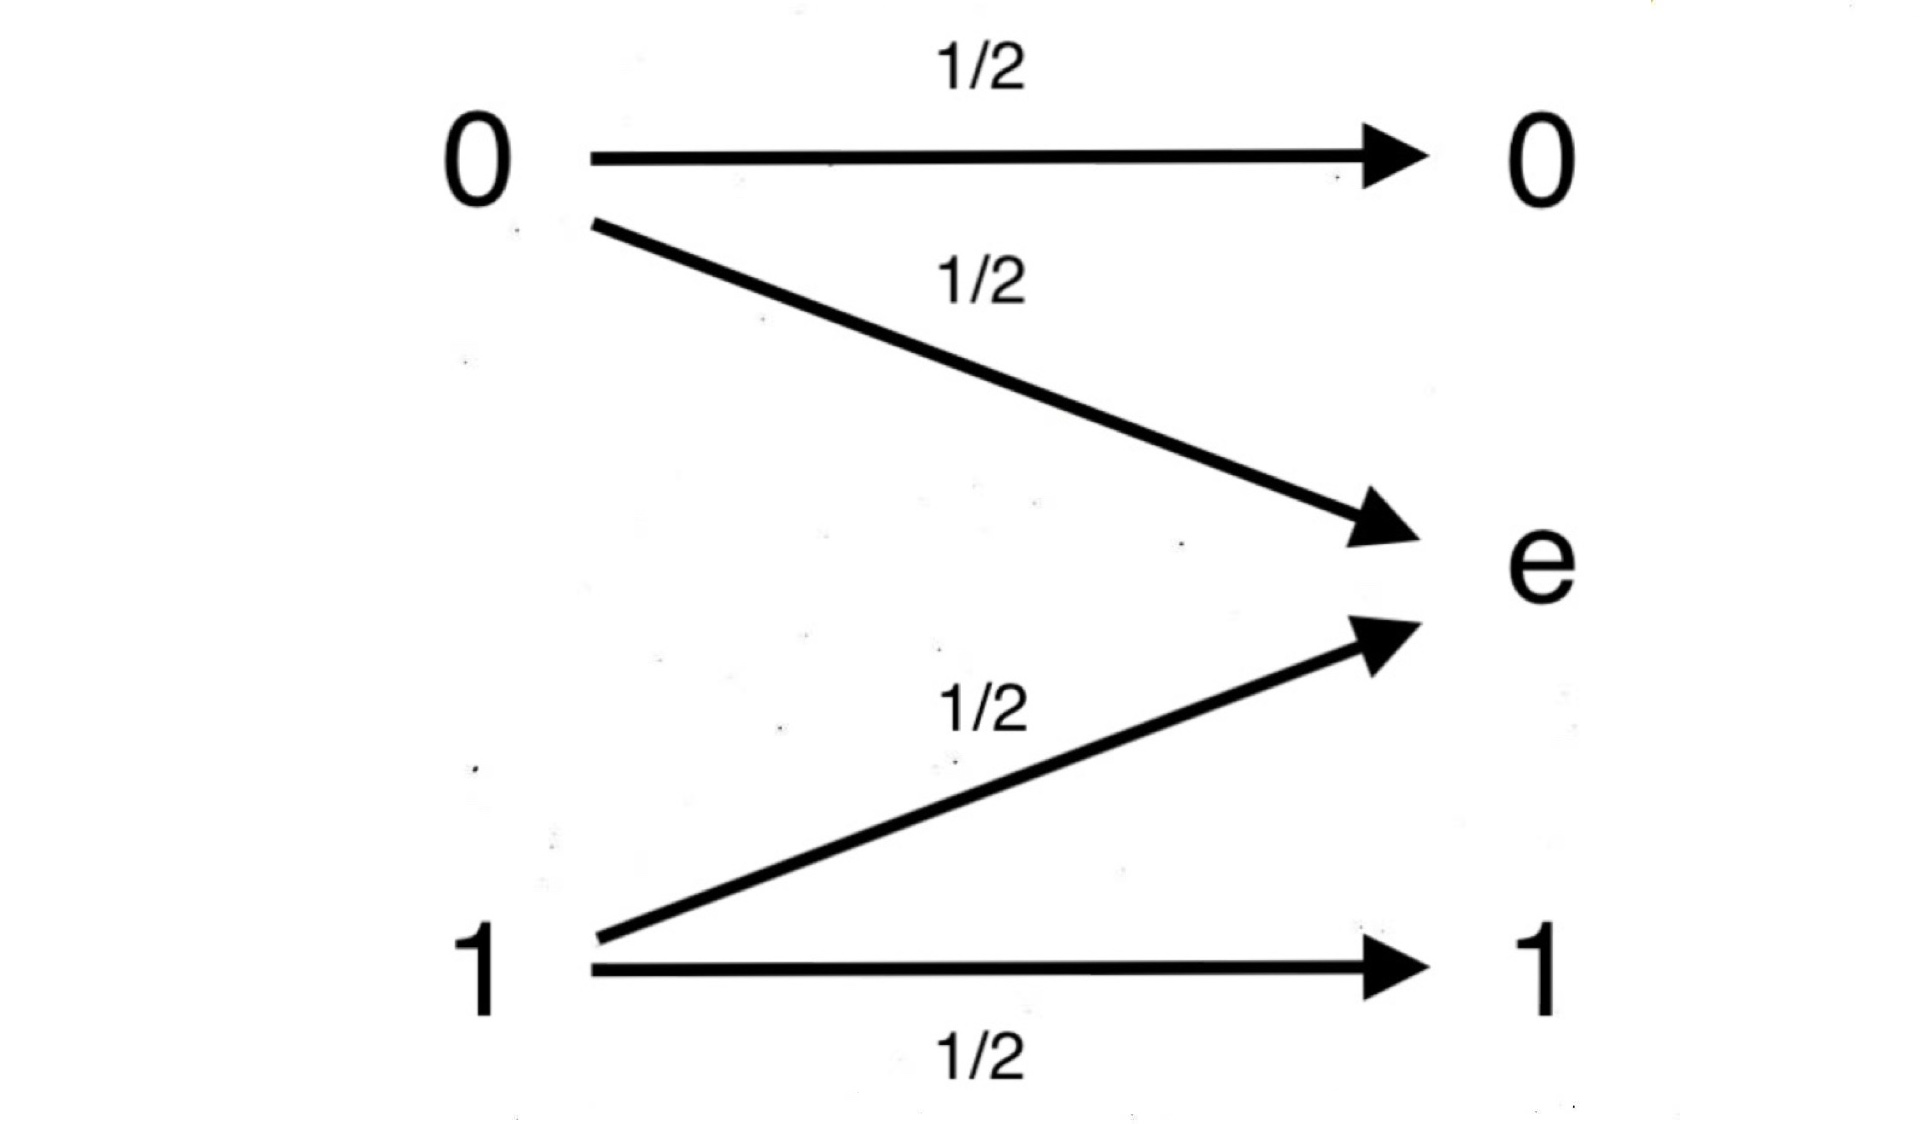
\includegraphics[width=0.4\textwidth]{Images/bec_bb84.jpg}
        \caption{BB84 channel model (withouth eavesdropping).}
     \label{fig:quadtree}
\end{figure} 

The mutual information of this channel is $I(X,Y)_{BB84} = 0.5$, which means that
the public discussion between Alice and Bob has improved the efficiency of the channel.
The channel has the following probability matrix: 
\[\underbar{P}_{BB84} = \begin{bmatrix}
    1/2 & 0 & 1/2\\
    0 & 1/2 &  1/2 \\
\end{bmatrix}\] 
In this way we get a bit every 2 channel uses, as expected by the protocol. 
A more generalized version of this protocol exits, called the six-state protocol, adds the circular polarization to the possible basis. The circular basis introduces two more states: $\frac{1}{\sqrt{2}}\ket{0}+\frac{i}{\sqrt{2}}\ket{1}$ and $\frac{1}{\sqrt{2}}\ket{0}-\frac{i}{\sqrt{2}}\ket{1}$, and the channel assumes the following probability matrix: 

\[\underbar{P}_{ssp} = \begin{bmatrix}
    1/3 & 0 & 2/3\\
    0 & 1/3 &  2/3 \\
\end{bmatrix}\] 

With source probabilities $P(X_i) = 1/2$, and channel model:

\begin{figure}[!h]
    \centering
    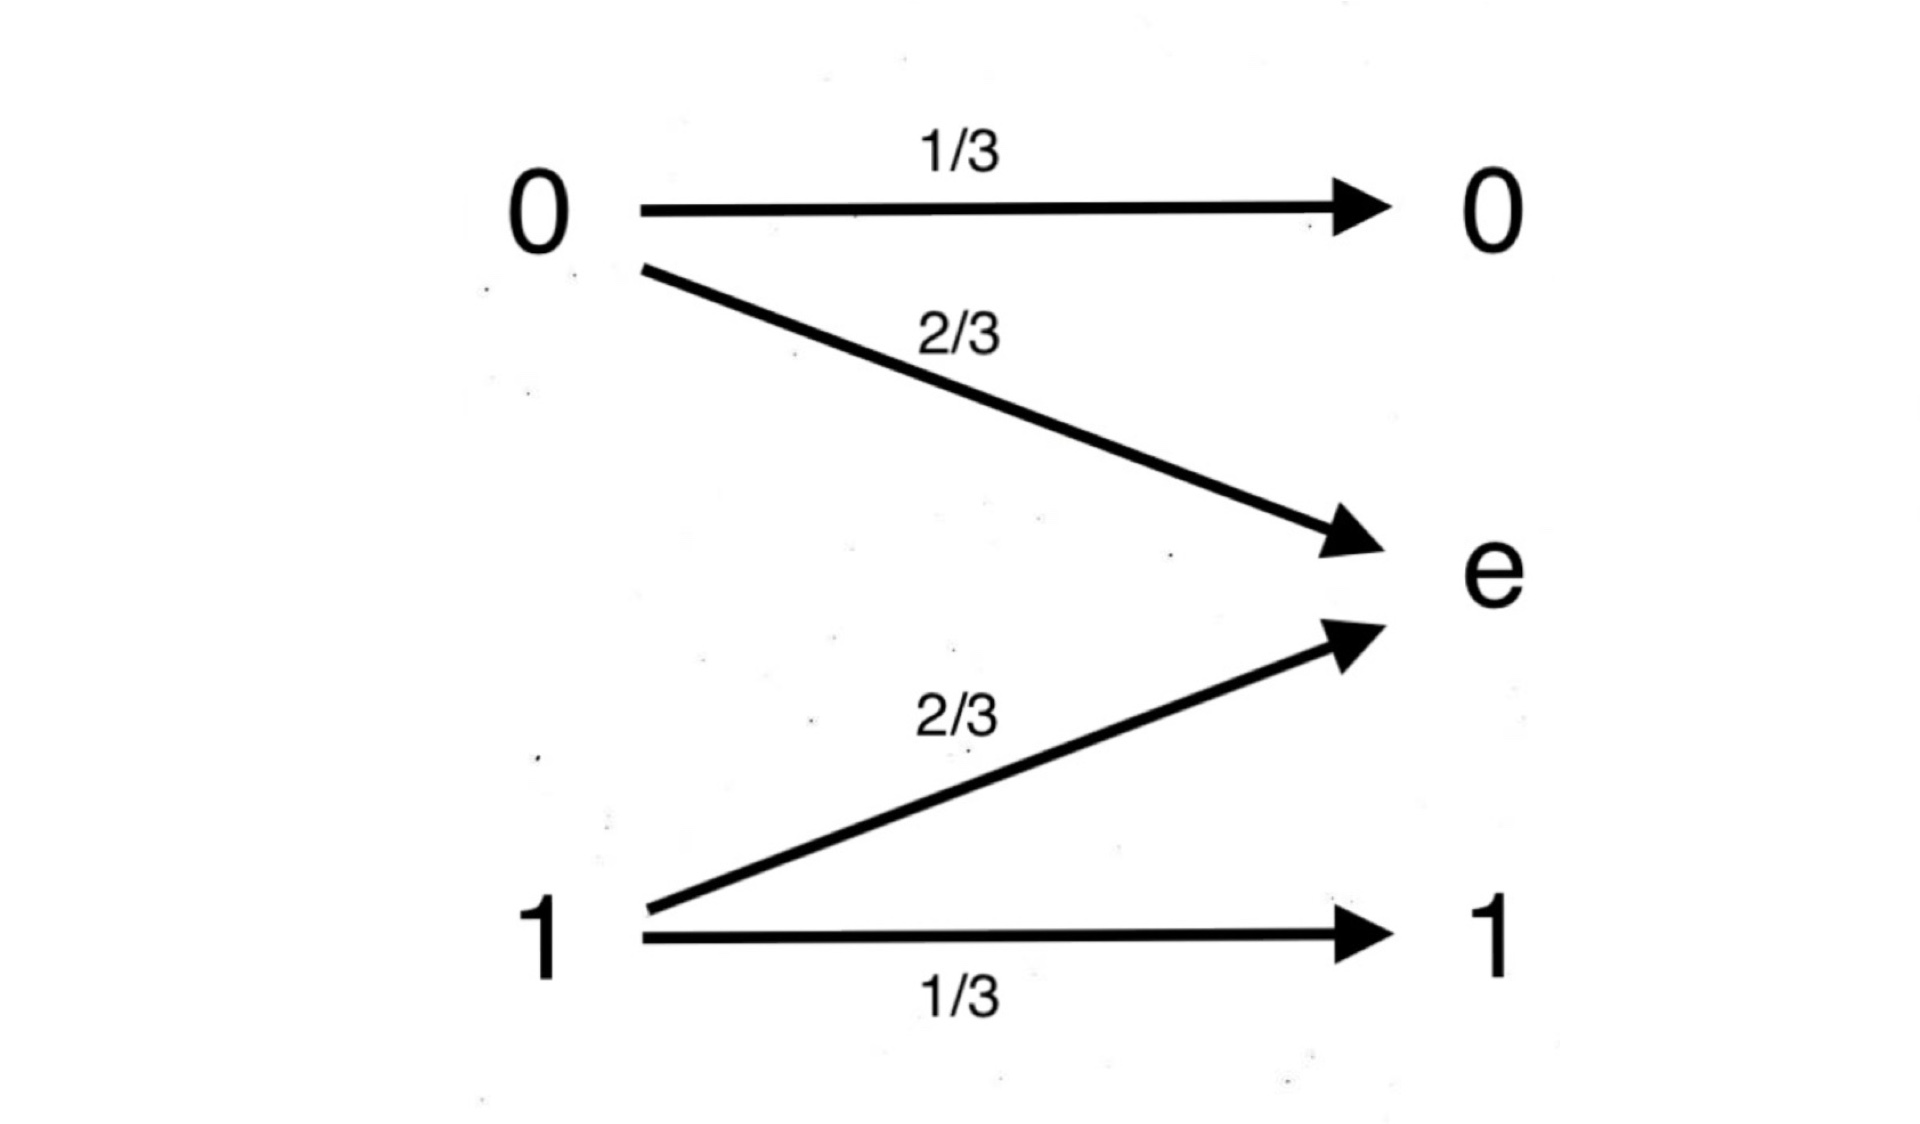
\includegraphics[width=0.45\textwidth]{Images/bec_ssp.jpg}
        \caption{Six-state protocol channel model (withouth eavesdropping).}
     \label{fig:quadtree}
\end{figure} 

This protocol achieves a lower mutual information: 

\[I(X,Y)_{SSP} = 1/3\]

We receive, on average, a bit for the secret key every 3 channel uses, which is worse than the BB84 protocol. However, as we will see in the following examples, the SSP trades it off for a better resilience against eavesdropping. 

\section{Discrete Variable QKD with eavesdropping}
Ideally, the sifted keys obtained by Alice and Bob should be the same, but in a real scenario we also have to consider the presence of an eavesdropper (Eve) and its effect on the channel capacity. It is a difficult task to bring together information theory and quantum mechanics, because they can be combined in several ways, depending on the protocol used and on the way the eavesdropping is performed. Therefore, we focus on a specific type of \textit{individual} attacks: the intercept-resend. 
Eve's task is to intercept all photons individually, to measure them, and to re-send them in the same state they were obtained. The intrusion of Eve can be noticed only when Bob chooses the same polarization basis as Alice, because otherwise the bit is discarded \textit{a priori}. When Eve re-sends a photon with the same basis as Alice and Bob, but in a different state, the bit received is flipped, and Bob notices the presence of the eavesdropper. For the BB84, we can implement the presence of Eve using the following channel model (source probabilities $P(X_i) = 1/2$): 


\begin{figure}[!h]
    \centering
    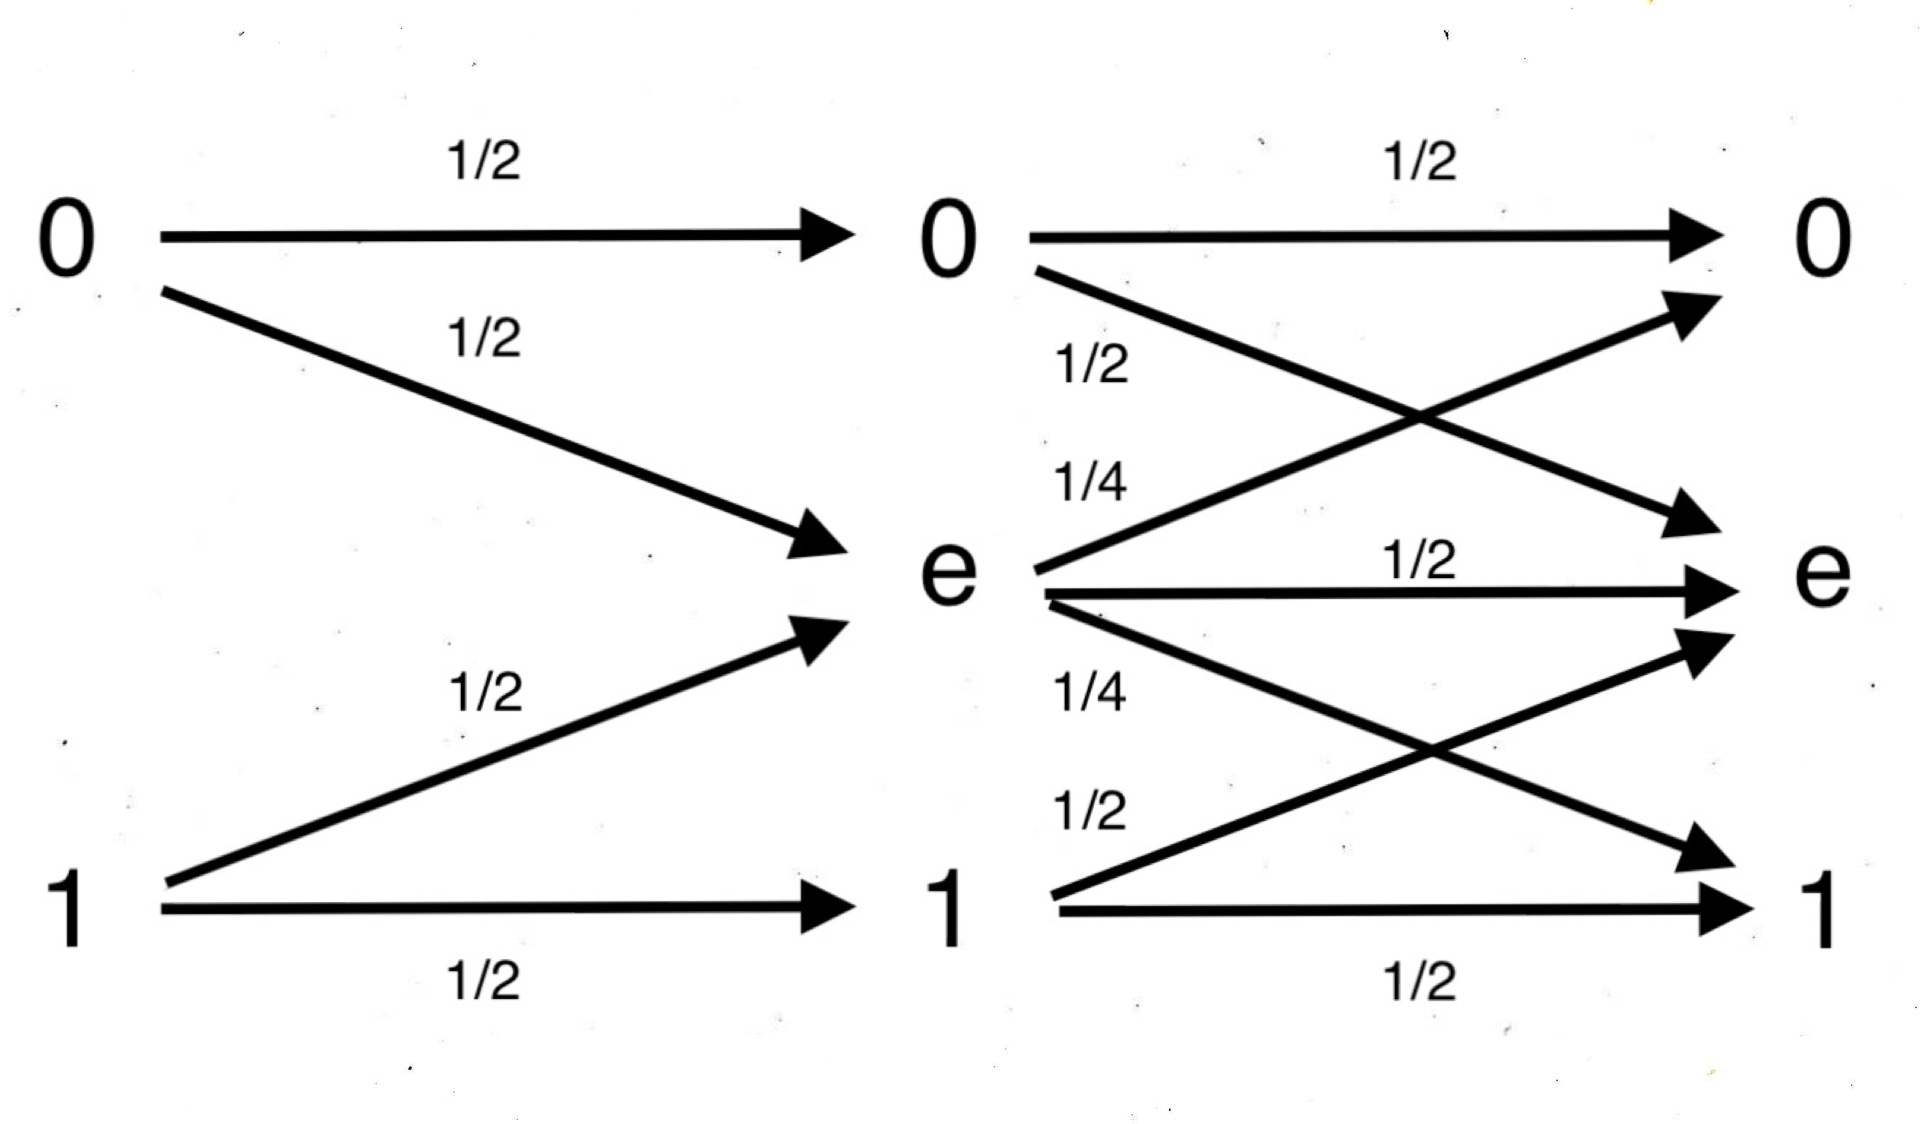
\includegraphics[width=0.5\textwidth]{Images/bb84_eve.jpg}
        \caption{BB84 channel model (intercept-resend attack).}
     \label{fig:quadtree}
\end{figure} 

We can calculate a quantity called Quantum Bit Error Rate (QBER), which is defined as the number of the wrong (flipped) bits of the sifted key over the length of the sifted key: 
\[QBER_{BB84} = \frac{P(y=1|x=0)}{P(y=0|x=0)+P(y=1|x=0)}=\]
\[= \frac{1/8}{(1/4+1/8)+1/8} = 1/4 = 25\%\]
Due to the errors, the sifted key shared between Alice and Bob is not the same anymore, so we need to apply an error correction code to have a perfect match between them. Furthermore, now Eve has knowledge of some bits of the secret key, so we need to apply a privacy amplification protocol to reduce its information. The information received by Eve is equal to the information of a channel without eavesdropping, so we use the result of the previous chapter: $I(X,Eve) = 0.5$. In order to calculate $I(X,Y)$, we need to define the probability matrix of the new channel model: 
\[\underbar{P}_{BB84,X\rightarrow Y} = \begin{bmatrix}
    3/8 & 1/8 & 1/2\\
    1/8 & 3/8 &  1/2 \\
\end{bmatrix}\] 
We obtain: $I(X,Y) = 0.0944$. We also calculate $I(Eve,Y) = 0.25$, considering the channel between Eve and Bob ($P(Eve=e)=1/2, P(Eve=0,1)= 1/4$): 

\[\underbar{P}_{BB84,Eve\rightarrow Y} = \begin{bmatrix}
    1/2 & 1/2 & 0\\
    1/4 & 1/2 &  1/4 \\
    0 & 1/2 & 1/2
\end{bmatrix}\] 

To verify whether we can apply error correction and privacy amplification to the sifted key, we use the Csiszár-Körner theorem\cite{cryptoreview,korner}: if $I(X,Y)\geq \min(I(X,Eve)$, $I(Eve,Y)) \Rightarrow$ a secret key can be obtained. In our case $I(X,Y)$ is lower than the other two mutual informations, however, we have to consider that Eve isn't always present in the channel, so the real capacity is an average between the channel with and without eavesdropping. We define a new variable $\mu$, as how many photons are intercepted by Eve over the number of photons sent by Alice. We calculate the minimum $\mu$ for which the Csiszár-Körner theorem is fulfilled (how much Eve can interfere), taking as lower bound $I(Eve,Y)=0.25<I(X,Eve)$: 

\[I(X,Y)_{no,Eve}(1-\mu)+I(X,Y)_{Eve}\cdot\mu \geq I(Eve,Y)\]

\[0.5(1-\mu)+0.0944\mu \geq 0.25\]

\[\Rightarrow \mu_{BB84} \leq 0.6164\]

Therefore, the maximum QBER tolerated by the BB84 is: 

\[QBER_{MAX,BB84} = QBER_{BB84}\cdot \mu = (25\%)\cdot0.6164 \simeq 15.4\% \]

Which is analogous to the result obtained by Gisin et al. \cite{cryptoreview}.
\\
\\
The same procedure can be applied to analyze the six-state protocol, which has the following channel model:

\begin{figure}[!h]
    \centering
    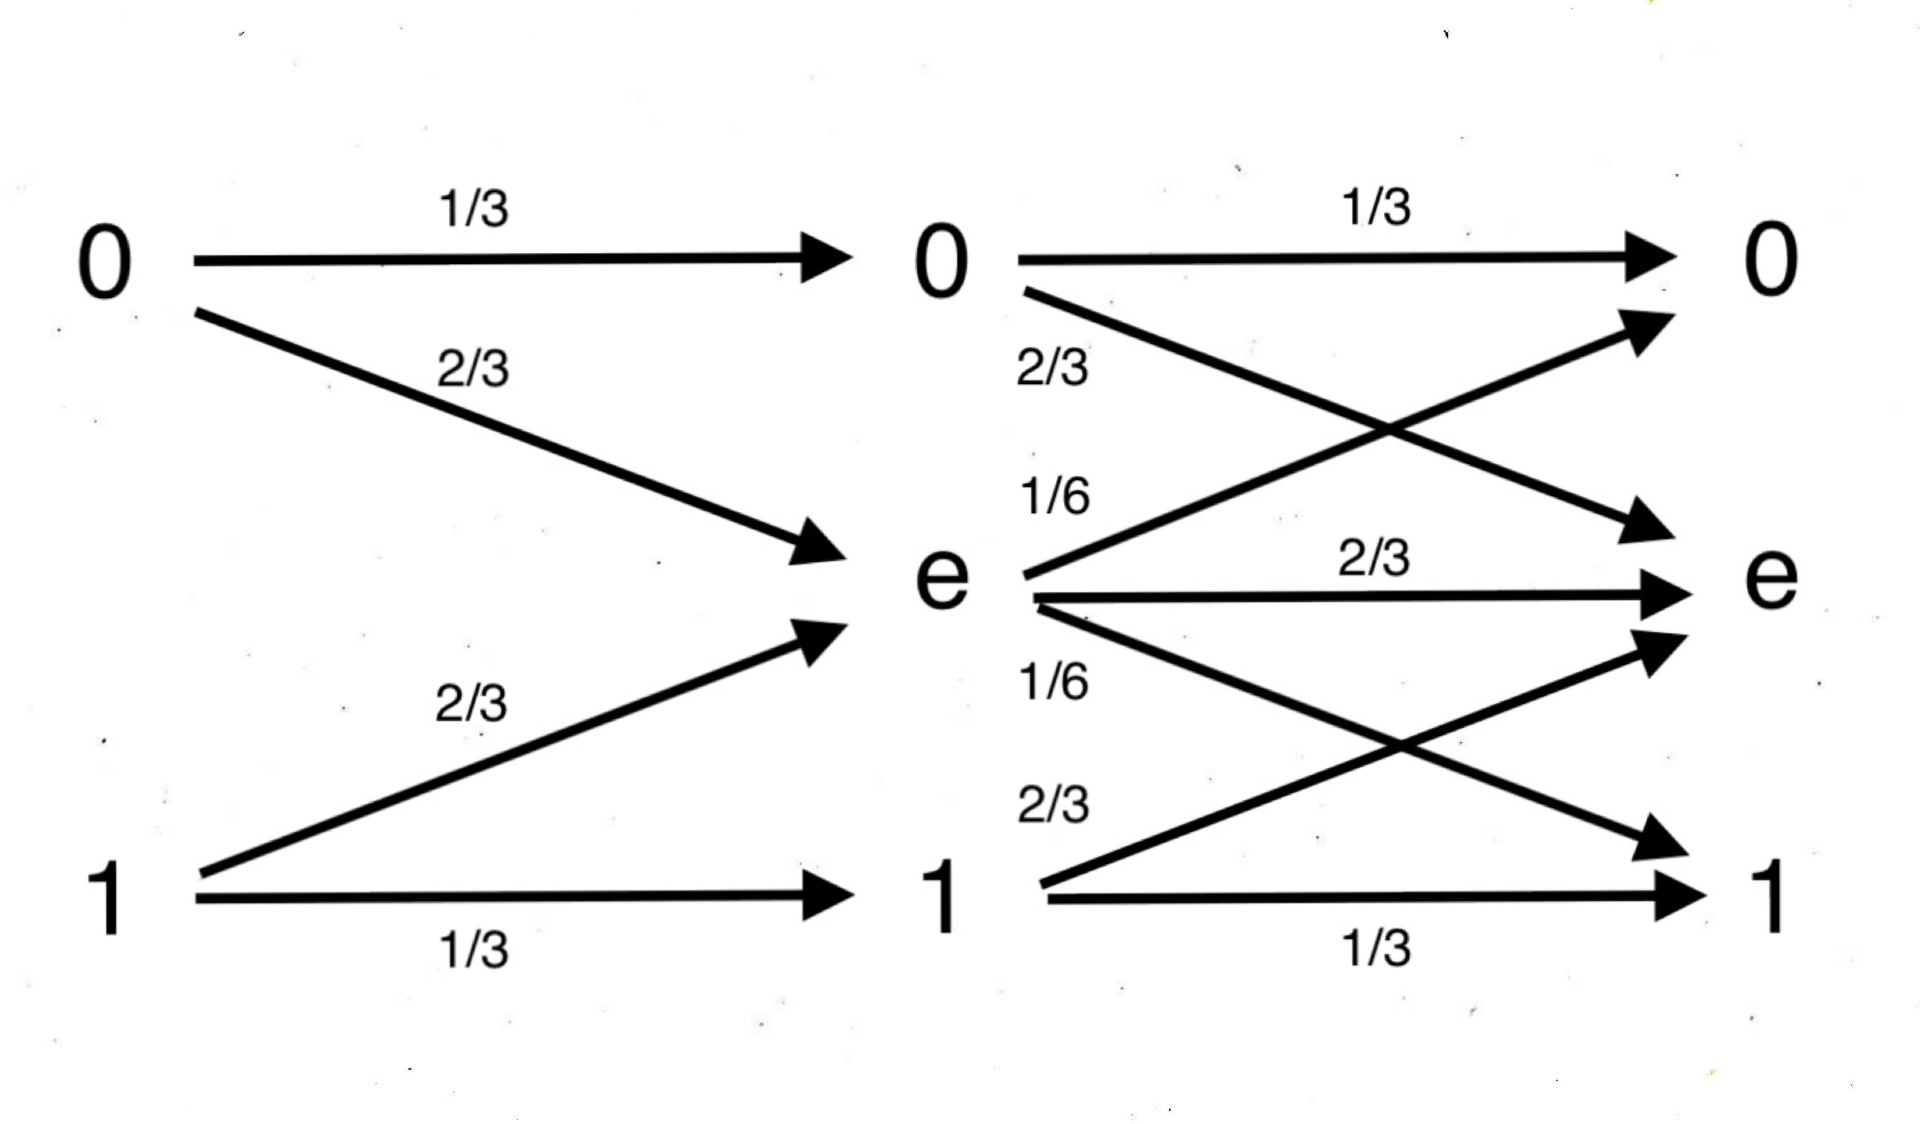
\includegraphics[width=0.5\textwidth]{Images/ssp_eve.jpg}
        \caption{six-state protocol channel model (intercept-resend attack).}
     \label{fig:quadtree}
\end{figure}

And probability matrix: 

\[\underbar{P}_{SSP,X\rightarrow Y} = \begin{bmatrix}
    2/9 & 2/3 & 1/9\\
    1/9 & 2/3 &  2/9
\end{bmatrix}\] 
\\
We obtain $I(X,Y) = 0.0272$ (source probabilities $P(X_i) = 1/2$) and a QBER: 
\[QBER_{ssp} = \frac{2/18}{(1/9 + 2/18) + 2/18} = 1/3 = 33.3\% \]
The maximum QBER for the six-state protocol is found applying again the Csiszár-Körner theorem. As a first step, we calculate the other mutual information: $I(X,Eve) = 1/3$, it is the same as a channel without eavesdropping, and $I(Eve,Y) \simeq 0.1111 $ is obtained using the following probability matrix (Eve probabilities $P(Eve = e) = 2/3$, $P(Eve = 0,1)=1/6$):

\[\underbar{P}_{SSP,Eve\rightarrow Y} = \begin{bmatrix}
    1/3 & 2/3 & 0\\
    1/6 & 2/3 &  1/6\\
    0 & 2/3 & 1/3
\end{bmatrix}\] 
Applying the theorem, we find:

\[(1/3)(1-\mu)+0.0272\mu \geq 0.1111\]

\[\Rightarrow \mu_{ssp} \leq 0.7259\]
\[\Rightarrow QBER_{MAX,ssp} = (33.3\%)\cdot0.7259 \simeq 24.2\% \]
This is a higher value than the maximum QBER of BB84, so we have quantitatively demonstrated that the six-state protocol is more resilient against intercept-resend attacks. 
\\ 

\section{Continuous-Variable QKD}
As we have shown in the previous paragraph for the specific case of intercept-resend attack, discrete-variable QKD is not hard to analyze in terms of capacity and QBER. However, it is not an easy task to realize an experimental implementation of this category of protocols, because they require single-photon sources (usually approximated with weakly coherent beams) and direct detection. Alternatively, it is possible to use continuous variables of the quantized electromagnetic field, such as its amplitude and phase, to encode the information. In this case, we just need to produce coherent states of light and to use homodyne detection, which is easier and more efficient than the DV-QKD setup. In this new setting, the concept of qubit, or more in general, qudit, loses significance, and we use the analogue concept of qumode, a quantum state in an infinite Hilbert space. Each mode of this space can be described by the quadrature field operators, $\hat{q}$ and $\hat{p}$. These two operators don't commute, and using the (generalized) Heisenberg uncertainty principle we get a relationship for their variances \cite{wolf,griffiths}: 
\[\sigma_q^2\sigma_p^2 \geq N_0\]
Where $N_0$ is the shot noise. This means that we can't measure with the same probability both quadratures with arbitrary precision. This result changes the points of the p-q plane 
of a coherent state into circles: 

\begin{figure}[!h]
    \centering
    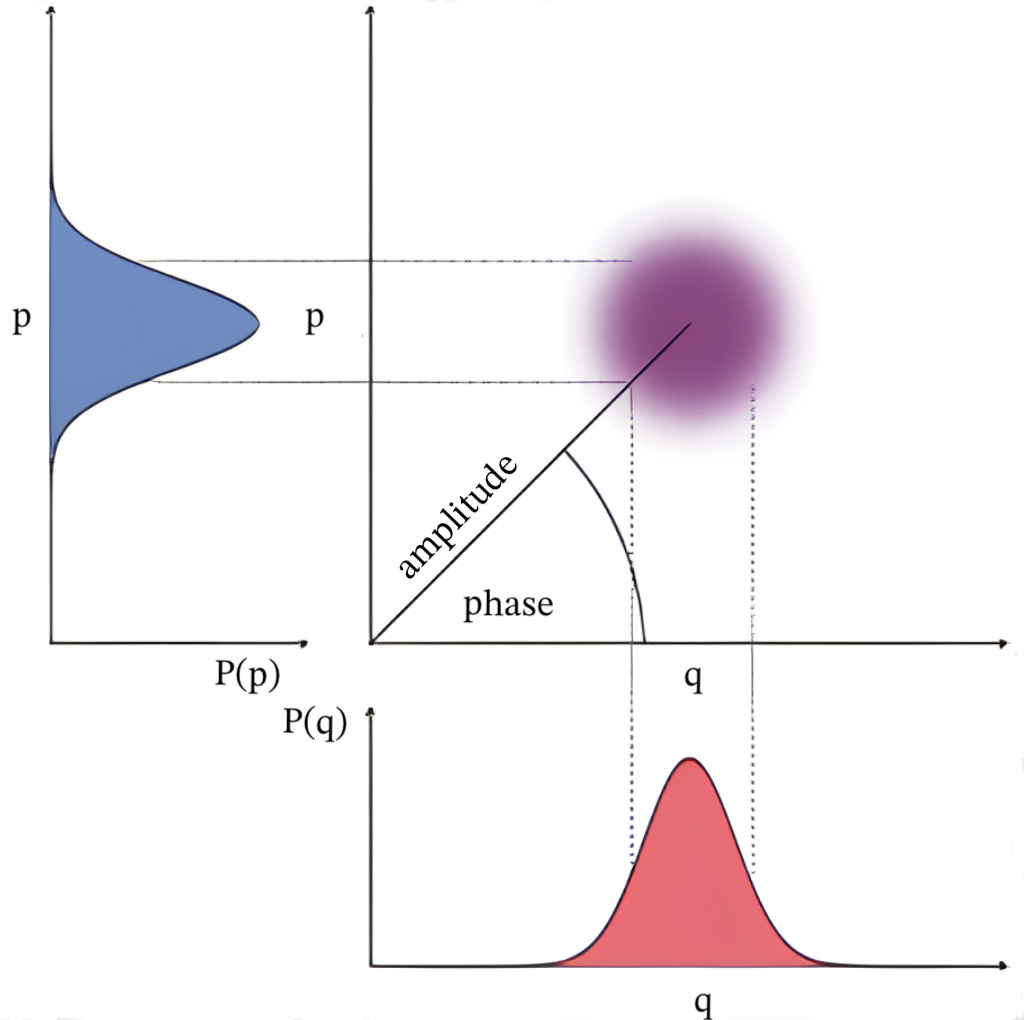
\includegraphics[width=0.5\textwidth]{Images/blur.png}
        \caption{Coherent state with Gaussian Wigner function \cite{wolf}.}
     \label{fig:quadtree}
\end{figure}

Each quantum state can be described by a quasi-probability distribution (Wigner function) which is analogous to the density operator used for qudit systems. Coherent states of light are Gaussian states, this means that they have a Gaussian Wigner function. 
We're particularly interested in these states because it is known how to generate them with lasers. Morover, also Fock states, which are light pulses in a state with an exact number of photons, are Gaussian states, and as it will be shown in the next paragraph, Gaussian modulated Fock states set the maximum capacity obtainable in Bosonic Gaussian channels. 
%https://physics.stackexchange.com/questions/305226/which-state-to-use-fock-coherent
The simplest CV-QKD protocol that exploits coherent states is the GG02 \cite{grosshans}, and it resembles in some features the BB84 protocol: Alice prepares a finite number of coherent states $\ket{q + ip}$, picking them from a complex Gaussian probability distribution with zero mean and variance $V$. The states are sent to Bob, which measures at random one of the quadrature with homodyne detection. The measurement is optimal, which means that the variance added is just equal to the (intrinsic) shot-noise $N_0$. We can also consider other noise parameters  such as transmission efficiency $\tau$ and excess noise $\xi$ (channel noise), and quantum efficiency $\eta$ and electric noise $v_{el}$ (non-ideal detection noise). The Gaussian variable received by Bob is the sum of one of the variables sent by Alice, $X_{A}$, with the Gaussian noise variable $X_{N}$ with variance $V_{N} = N_0 + \eta\tau\xi+ v_{el}$ and zero mean \cite{jouguet}:
\[X_{B} = \sqrt{\eta\tau}(X_{A}+X_{N})\]
With variance: 
 \[V_{B} =\eta\tau V_{A} + V_{N}\]
Using a classical public channel, Bob informs Alice about which quadrature was measured, and about half of the key is discarded. 
The steps remaining consist in the classic post-processing. It includes, similarly to DV-QKD, error correction, parameter estimation and privacy amplification. 
\\
\\
To simplify the analysis of the protocol in terms of key extraction, information rate and QBER, it's convenient to use a discrete modulation of coherent states. In the last paragraph, we will show an implementation of of the GG02 protocol, using a discrete alphabet of symbols-states whose constallation is shaped on a Gaussian distribution \cite{Roumenstan}.

\section{Holevo's bound in Optical Communications}
In this paragraph we want to show that it's possible to improve the capacity of a channel by switching from a classical encoding of information to a quantum one. So far we have seen that it's not possible to overcome the Shannon's entropy of memory-less stationary source. In real-case scenarios a communication channel is never lossless, and noise modifies the maximum amount of information per channel use that can be reliably communicated. An usual channel model used in optical communication is the AWGN (Additive White Gaussian Noise) channel, in which the noise is considered independent from the input of the channel. Its capacity is computed by finding the maximum of the mutual information all over the possible input distributions, which in the classical case is demonstrated to be also a Gaussian distribution: 
\[C = \max_{\{P(X)\}}{I(X,Y)} = \frac{1}{2}\log(1+SNR) \]
The SNR is the signal to noise ratio, the average power of the input signal over the average power of the noise. It is possible to use this model to calculate the capacity of an optical communication channel that uses a linearly polarized optical signal in two-quadrature encoding\cite{banaszek,gordon} and homodyne detection:
\[C_{S2} =\log(1+ \frac{n_s}{n_n+1})\]
This capacity is in function of the average received signal photon number ($n_s$) and the mean number of excess noise photons ($n_n$) per temporal slot. This approach is semi-classical and doesn't use quantum states to encode the information. However it possible to demonstrate that the same result holds for coherent states of light, which are the quantum counterpart of the semi-classical approach\cite{semic}. Otherwise, it is possible to encode the information in quantum (Fock) states of light containing an average number $\bar{n} = n_s$ of photons with probability $p_n$. In this case, the mutual information of the channel in absence of excess noise, and using an ideal photodetector is \cite{gordon}: 
\[I(x,y) = -\sum_n^{\infty} p_n\log(p_n) \]
Which only needs to be optimized with the physical constraint of conservation of average power (otherwise the best probability would be all equal probabilities, which is physically impossible): $\sum_n^{\infty} np_n = n_s$, to obtain the capacity (or accessible information): 
\[C_{F} = (n_s+1)\log(n_s+1)-n_s\log(n_s)\] that is an higher capacity than $C_{S2}$. 
The ensemble of Fock states can be rewritten in the formalism of the previous chapters using the density operator: 
\[\rho = \begin{bmatrix}
    p_1 & 0 & \dots & 0\\
    0 & p_2 &  &  \\
    \vdots &  & \ddots &  \\
    0 &  &  & p_n
\end{bmatrix}\] 
 If we now consider Gaussian noise, after propagating through the channel the quantum states will not be orthogonal pure states, but more general non-orthogonal mixed states, depending on the noise and on the input distribution.
 The minimum Holevo's quantity at the output of a Bosonic Gaussian Channel (quantum version of AWGN) is achieved by Gaussian input states \cite{giovannetti}. If we say that we can perform the best possible measure, the accessible information is equal to the Holevo's quantity, and the following formula is found: 
\[\chi = C_{H} = C_{F}(n_s+n_n)-C_{F}(n_s)\]
  Comparing this result with the classical capacity, we notice that $C_{H}\gg C_{S2}$ only when the excess noise is very low (in that case $C_{H} \simeq C_{F}$) and the average number of photons is not high enough (in that case $C_{H} \simeq C_{S2})$. However, it has not yet been found the right optical detection scheme for which the accessible information is equal to the Holevo's bound. We can conclude that, in non-ideal/real case scenarios, we don't get a higher capacity with Fock states, especially when the mean number of photons ($n_s$) is high enough. 

\section{Channel Model and Simulations}
%Using the theory developed in the previous paragraphs, we will analyze through simulations the information rate and the QBER of the GC02 protocol. 
In practice, to implement the GC02 protocol, the input and output constellations are usually discretized. Although this does not impact the security capabilities of the protocol\cite{Ghorai}, using a lower cardinality constellation intrinsically limits the information (bit) rate of the protocol. Following the example of\cite{Roumenstan}, we sought to investigate the information rate of the GC02 protocol using high-cardinality QAM constellations, simulating the various distortion effects of the optical channel and receiver.
As for the input probability distribution, we follow the work of Roumestan et al.\cite{Roumenstan}; each symbol has probability:
\[P_X (p +iq) = \frac{e^{-v(p^2 + q^2)}}{\sum_{p,q} e^{-v(p^2 + q^2)}} \]
where $p$ and $q$ are, respectively, the in-phase and in-quadrature components of the symbol. \\
\\
Various effects can disturb an optical signal that is propagating through a fiber. Attenuation, due to scattering and absorption, weakens the propagating signal, and dispersion broadens the pulse width. The last effect can cause inter-symbol interference after a certain distance, meaning that the receiver will no longer correctly distinguish the symbols because they are overlapped:
\begin{figure}[!h]
    \centering
    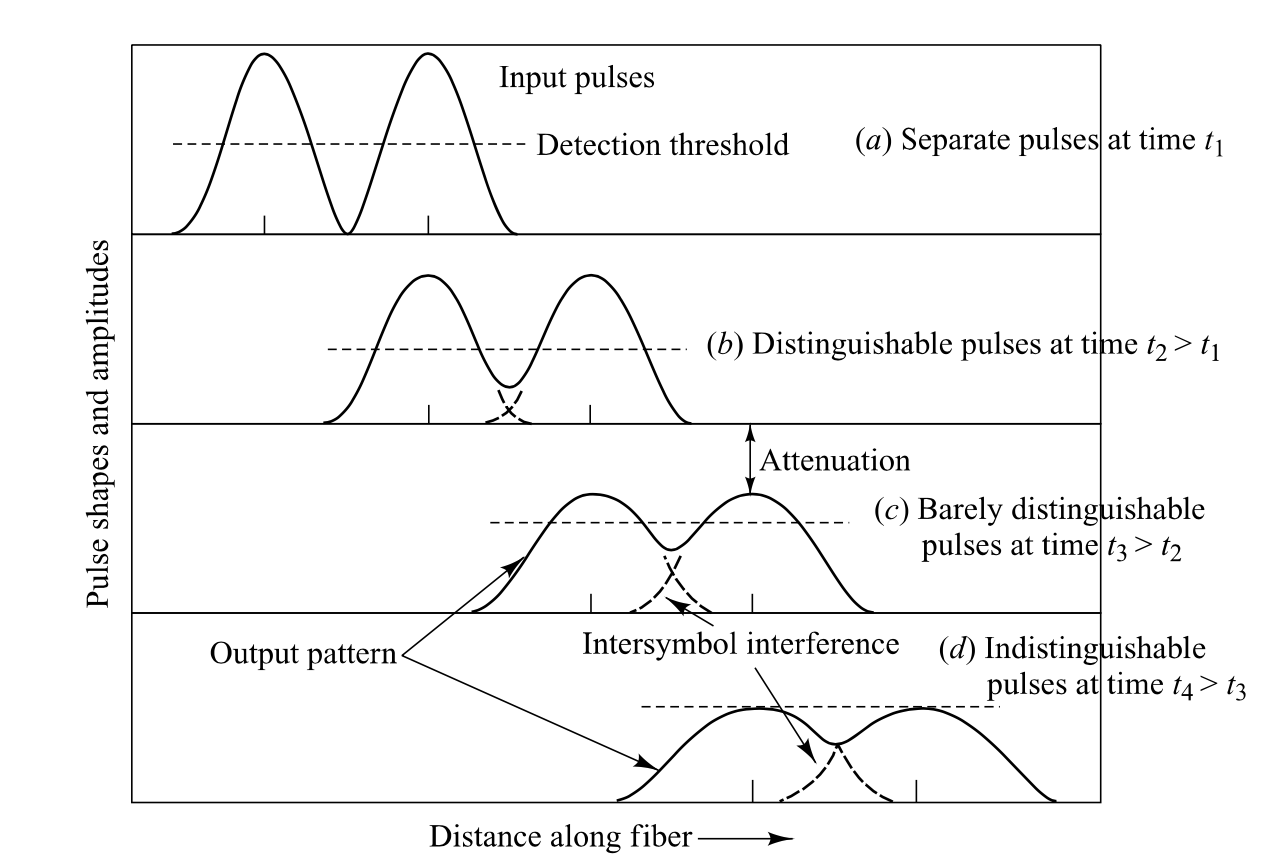
\includegraphics[width=0.5\textwidth]{Images/dispersion_effect.png}
        \caption{Example of the effect of chromatic dispersion on two consecutive symbol\cite{keiser}.}
     \label{fig:quadtree}
\end{figure}
Consequently, we obtain a higher bit error rate and a worse capacity. Chromatic dispersion results from the group velocity being a function of the wavelength, so the distortion increases with a large spectral band of the light source. It depends on both waveguide dispersion and material dispersion. The first one is the consequence of shorter wavelengths being more confined in the fiber core, so their effective refractive index is more similar to the index of the core, thus changing the beta; material dispersion is caused by the refractive index of the material being a function of the wavelength. We can model our propagation constant by expanding it with a Taylor series \cite{keiser}:
\[\beta \simeq \beta_0(w_0) + \beta_{1}(\omega-\omega_0) + \frac{1}{2}\beta_2(\omega-\omega_0)^2\] 

The factor $\beta_2 =\frac{ \partial^2\beta}{\partial\omega^2}$ is the group velocity dispersion (GVD) and it is related to the dispersion: 
\[D = -\frac{2\pi c}{\lambda^2}\beta_2\]
which is the result of both the material and the waveguide dispersion. 
\begin{figure}[!h]
    \centering
    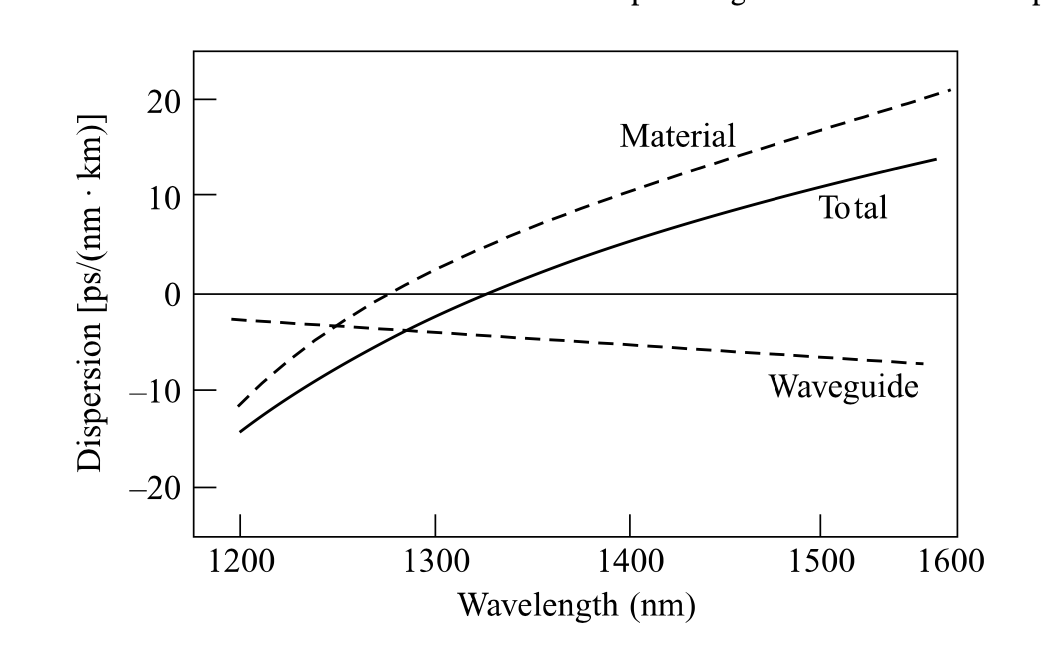
\includegraphics[width=0.5\textwidth]{Images/dispersion_scheme.png}
        \caption{D as function of the wavelength. For a standard mono-mode fiber operating in the C band (1550 nm) D is equal to 17 ps/(nm*km)  \cite{keiser,essiambre}.}
     \label{fig:quadtree}
\end{figure}
\\
\\
Chromatic dispersion is one of the main limiting factors in optical communication systems and it has to be accounted for, either at the physical level using dispersion compensating systems such as gratings fiber and special \textit{dispersion-compensating fiber}, using standard single-mode fibers in the O-band, or by compensating it with digital signal processing.
\\
\\
Another relevant source of noise inside an optical channel originates from the use of optical amplifiers: usually made with erbium-doped glass, they act as a source of non-coherent light, reducing the SNR and changing the statistics of the photo-counting at the receiver from a Poissonian to a Laguerre-Gauss distribution\cite{LagMartinelli}. However, as mentioned in the previous paragraph, we have chosen not to include optical amplifiers within our model. The reason is that the increase in noise which amplifiers introduce is not compatible with the high-cardinality constellation we want to obtain, and it would limit the maximum length of the optical channel. Furthermore, even if non-linear effects are relevant in coherent detection systems\cite{essiambre}, we have not included them in our model since the average power used by our source is in the order of some photons. 
\\
\\
Another aspect that must be taken into account in coherent detection systems is phase noise. Generally, coherent detection is influenced by three factors: phase noise in the local laser, polarization mismatch between the signal and the local laser, and multimode interference.
Polarization mismatch becomes relevant only for very high bit rate in long-haul links and can be managed using \textit{polarization diversity receivers}, and multimode interference can be avoided by a correct design of the receiver apparatus\cite{agrawal} or using a single-mode fiber, as in our case. Phase noise\cite{phasenoise}, on the other hand, is an intrinsic property of whatever laser may be used in our system \cite{orazio}, and as such it has to be included in the simulation of a coherent detection scheme. Starting from the linewidth $\Delta f$ and the power spectral density D of the laser being taken into account, we modeled the phase noise of the local laser with a Lorentzian power spectral density $S{(f)} \propto \frac{1}{f^2}$. 
\[
S{(f)} = \frac{A^2}{2\pi} \frac{\Delta f}{\Delta f^2 + f^2}
\]
The time samples of the phase jitter are then obtained filtering a Gaussian white noise and cumulating the result in the "phase" domain to obtain the random walk.

\begin{figure}[!h]
    \centering
    \includegraphics[width=0.5\textwidth]{}
        \caption{}
     \label{fig:quadtree}
\end{figure}

To approach these effects gradually, we begin our simulations by considering root raised cosine pulses with central wavelength $1550nm$, propagation without dispersion, phase noise and attenuation, and an ideal detector without dark counts and electrical noise ($\tau = 1,\eta = 1, \xi = 0, v_e = 0)$. The relevant effects that remain in the model are the variance of the Gaussian modulation and shot noise:
\[ X_B = X_A  +X_N \]
\[V_B = V_A + N_0 \]
We obtain the following information rate and QBER: 

\begin{figure}[!h]
    \centering
    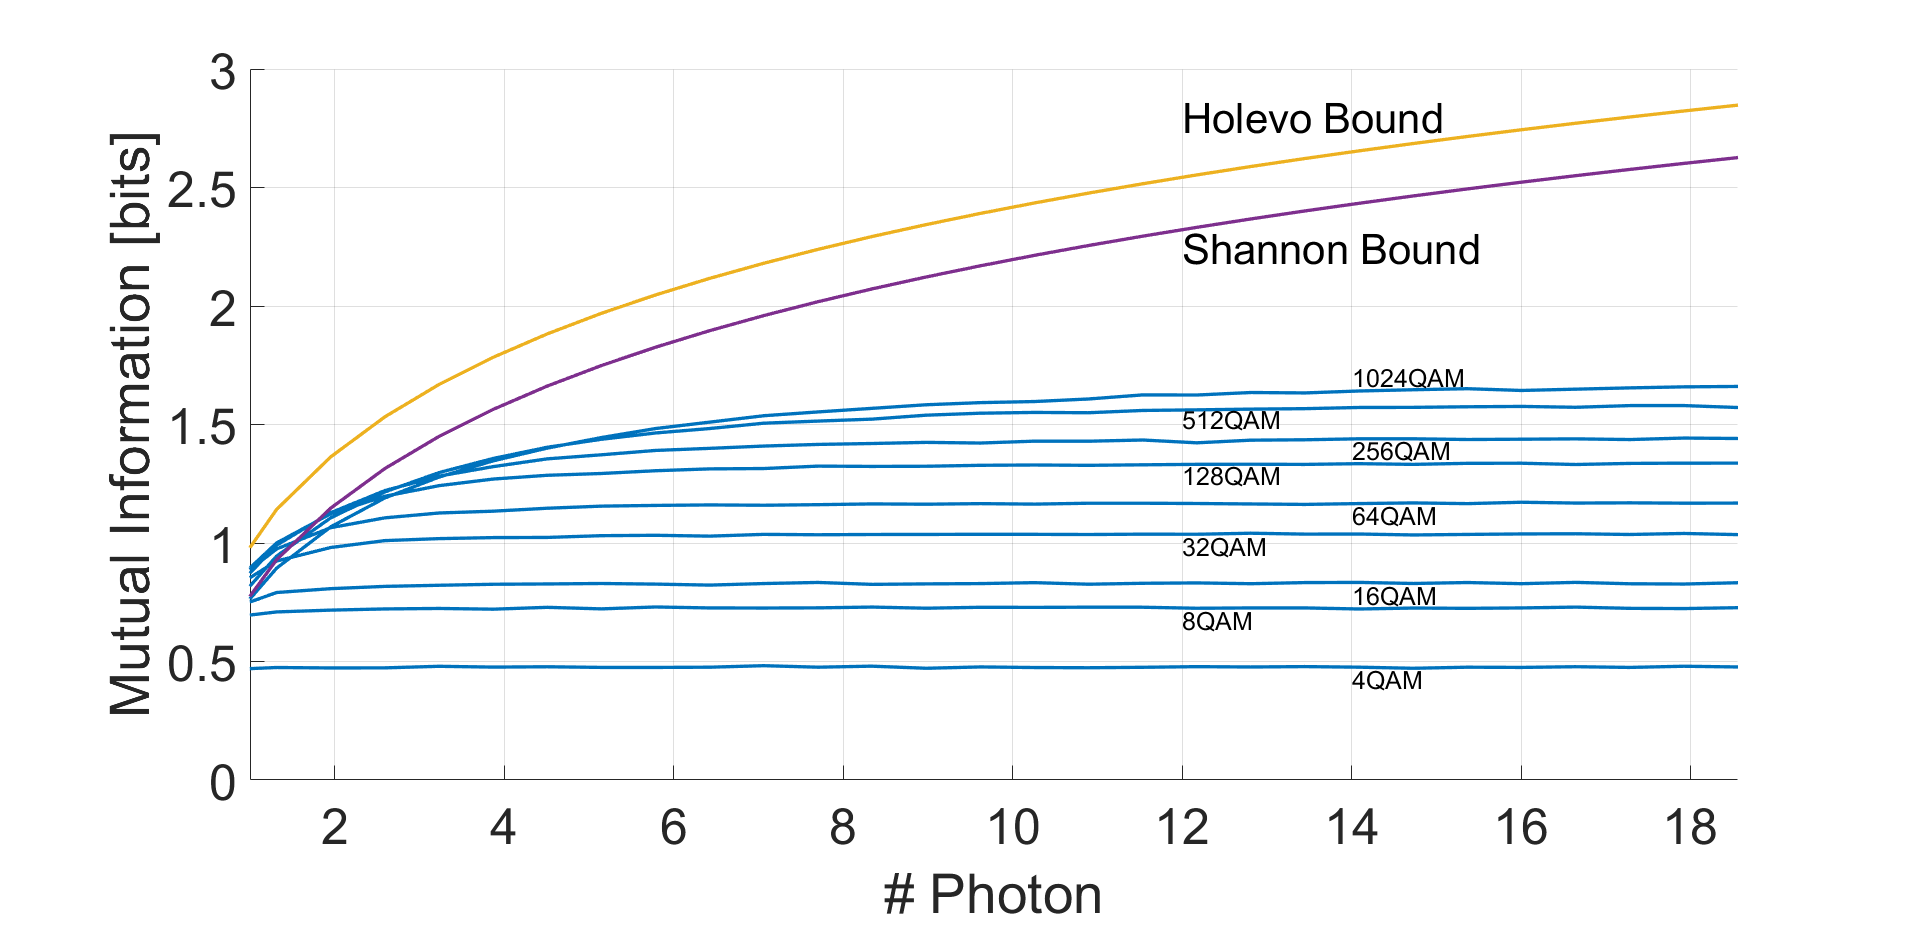
\includegraphics[width=\linewidth]{capacity_qber/capacity_example_2.png}
    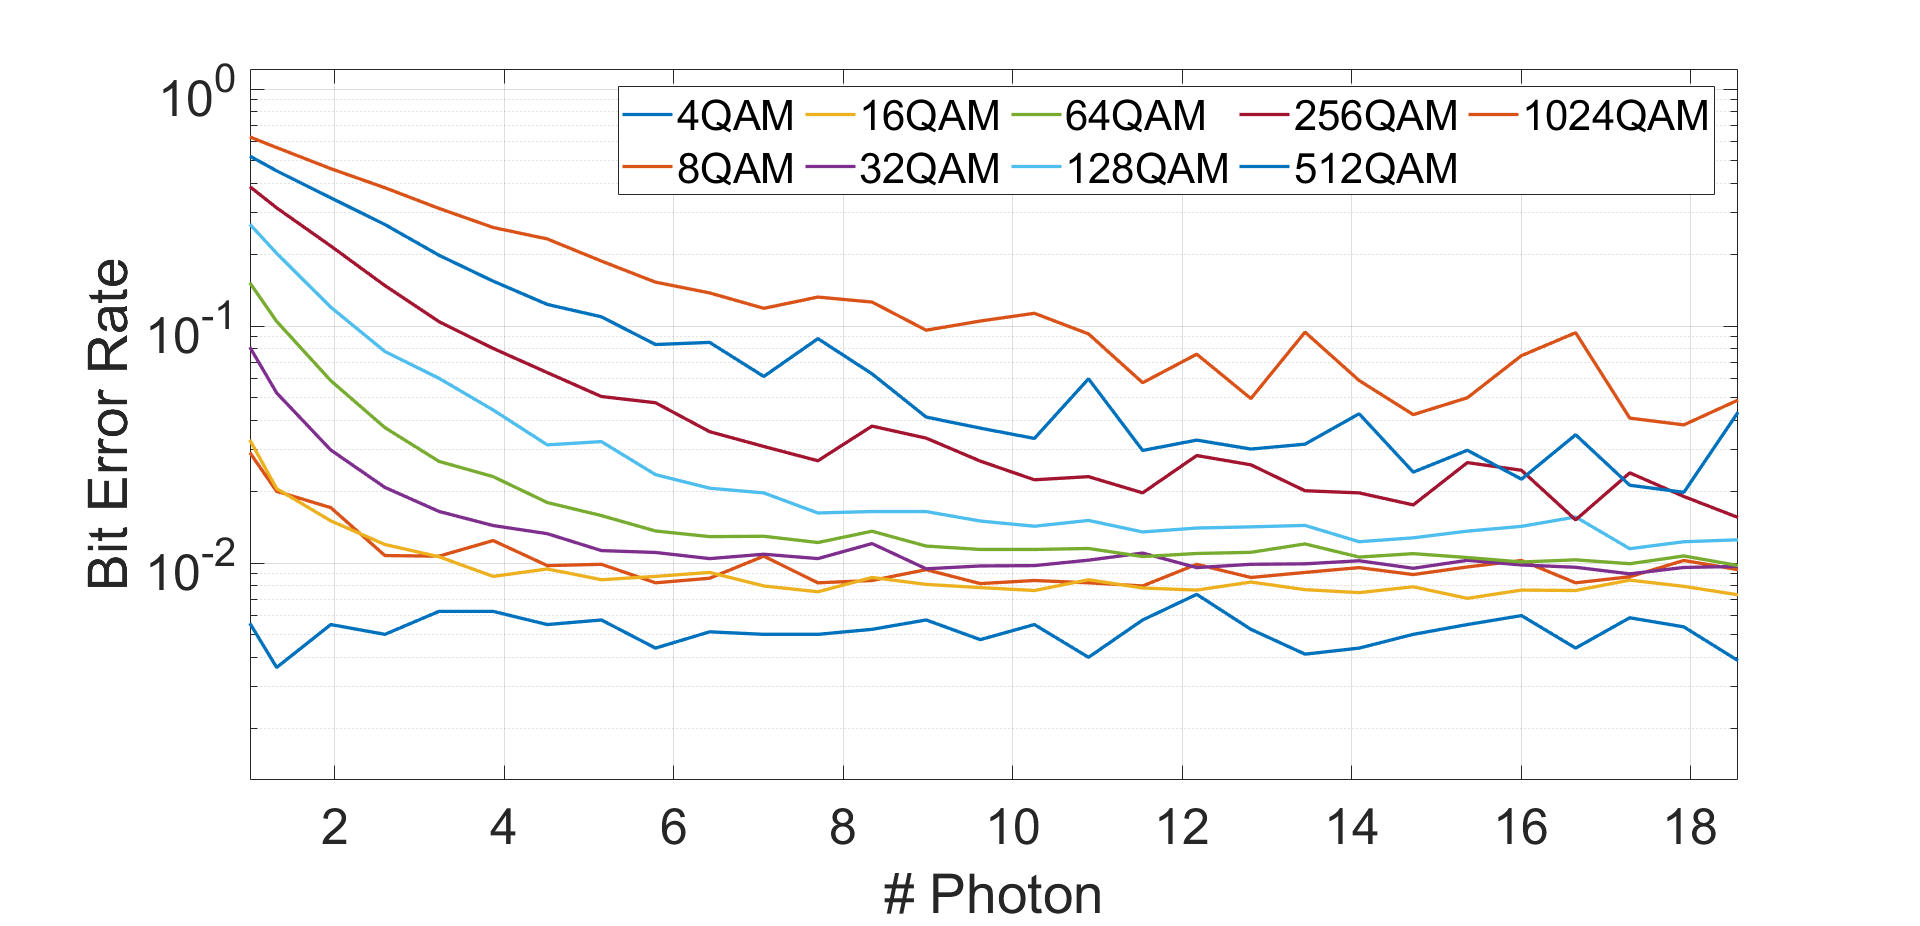
\includegraphics[width=\linewidth]{capacity_qber/error_rate_example.png}
    \caption{Mutual Information and (Quantum) Bit Error Rate of the various modulation formats.}
    \label{fig:enter-label}
\end{figure}

We immediately notice from these graphs that the discretization of the Gaussian constellation has had a severe impact on the information rate of the protocol. The rate is now constrained for high values of SNR (high number of photons), it tends to saturate to a constant value. Moreover, the rates shown in our graphs are halved due to the fact that on average the protocol discards half of the photons/bits to construct the sifted key. We can increase the rate with a higher number of symbols in the QAM modulation, but this also involves a higher QBER. For all types of modulation format, the QBER tends to reach zero as the number of photons is large enough. Furthermore, we have included in the first graph the curve given by the Fock states to give an idea of the ultimate (quantum) limit that is possible to reach. Since we are encoding the information in Coherent states, our ideal curve is the Shannon Curve, obtained with a continuous Gaussian input. To retrieve the bits at the output, we use a hard decoding technique. This type of decoding has been used to simplify the complexity of the system, so as to avoid the use of error correction and privacy amplification. However, the use of this approach increase the error rate of high cardinality constellation formats, which saturates the value of the information rate even with an high number of photons (high input power). This phenomenon can be observed directly on the graph by noticing that the amount of mutual information added when increasing the number of symbols tends to smaller values at each step. 


\begin{thebibliography}{3}

\bibitem{chuang}
M.A. Nielsen and I.L. Chuang, "Quantum Computation and Quantum Information", Cambridge University Press.
\bibitem{clone}
W.K. Wootters and W.H. Zurek, "A single quantum cannot be cloned", Nature, vol. 299, October 1982.
\bibitem{mixed}
Steven J. van Enk, "Mixed and pure states", notes of the course of quantum mechanics, University of Oregon, \url{https://pages.uoregon.edu/svanenk/solutions/Mixed_states.pdf}
\bibitem{caltech}
John Preskill, "Quantum Information Theory", notes of the course of quantum computation, California Institute of Technology, \url{http://theory.caltech.edu/~preskill/ph229/notes/chap5.pdf} 
\bibitem{john}
John Wright, "Lecture 18: Quantum Information Theory and Holevo’s Bound", notes of the course of Quantum Computation and Information, Carnegie Mellon University, \url{https://www.cs.cmu.edu/~odonnell/quantum15/lecture18.pdf}
\bibitem{peres}
Asher Peres and William K. Wootters, "Optimal Detection of Quantum Information", Physical Review Letters, vol. 66, no. 9, 04 March 1991.
\bibitem{banaszek}
Konrad Banaszek, Ludwig Kunz, Michał Jachura and Marcin Jarzyna, "Quantum Limits in Optical Communications", Journal of Lightwave Technology, vol. 38, no. 10, May 15 2020.
\bibitem{gordon}
J.P. Gordon, "Quantum Effects in Communications Systems", Proceedings of the IRE, vol. 50, September 1962.
\bibitem{giovannetti}
V. Giovannetti1, R. García-Patrón, N. J. Cerf and A. S. Holevo, "Ultimate classical communication rates of quantum optical channels", Nature Photonics, 21 September 2014.
\bibitem{magarini}
A. Singh, K. Dev, H. Siljak, H. D. Joshi and M. Magarini,
"Quantum Internet—Applications, Functionalities, Enabling Technologies, Challenges, and Research Directions",IEEE Communications Surveys \& Tutorials, vol. 23, iss. 4, 2021.
\bibitem{bb84}
Charles H. Bennett and Gilles Brassard, "Quantum cryptography: Public key distribution and coin tossing", International Conference on Computer Systems and Signal Processing, 1984.
\bibitem{moderncrypto}
Gilles Brassard, "Modern Cryptology", Lecture Notes in Computer Science, Springer-Verlag, 1988.
\bibitem{spin}
Alfredo Luis and Alfonso Rodil, "Polarization versus photon spin", Optics Express vol. 22, issue 2, pp. 1569-1575, 2014.
\bibitem{cryptoreview}
Nicolas Gisin, Gregoire Ribordy, Wolfgang Tittel, and Hugo Zbinden, "Quantum cryptography", Reviews of Modern Physics, Vol. 74, January 2002.
\bibitem{korner}
I. Csiszar and J. Korner, "Broadcast channels with confidential messages", IEEE Transactions on Information Theory, vol. 24, Issue: 3, May 1978.
\bibitem{wolf}
Ramona Wolf, "Quantum Key Distribution: an introduction with exercises", Lecture Notes in Physics, vol. 988, 2021.
\bibitem{griffiths}
David J. Griffiths and Darrel F. Schroeter, "Introduction to Quantum Mechanics", Cambridge University Press, cap. 3, 2018.
\bibitem{grosshans}
F. Grosshans and P. Grangier, "Continuous Variable Quantum Cryptography Using Coherent States",  Physical Review Letters, vol. 88, num. 5, 4 February 2002.
\bibitem{recon}
G. Van Assche, J. Cardinal and N.J. Cerf, "Reconciliation of a quantum-distributed Gaussian key", IEEE Transactions on Information Theory, vol. 50 iss. 2, February 2004.
\bibitem{cvqkd}
F. Laudenbach, C. Pacher, Chi-Hang Fred Fung, A. Poppe, M. Peev, B. Schrenk, M. Hentschel, P. Walther and H. Hübel, "Continuous-Variable Quantum Key Distribution
with Gaussian Modulation—The Theory of Practical
Implementations", Advanced Quantum Technologies,
vol. 1, iss. 1, August 2018.
\bibitem{semic}
E. C. G. Sudarshan, “Equivalence of semiclassical and quantum mechanical descriptions of statistical light beams”, Physical Review Letters, vol. 10, pp. 277–279, April 1963.
\bibitem{keiser}
G. Keiser, "Fiber Optic Communications", cap. 3, Springer, 2021.
\bibitem{agrawal}
Govind P. Agrawal, "Fiber-Optic Communications Systems", cap 7 and 10, Wiley 2002.
\bibitem{fibtoolbox}
Kotya Karapetyan, Optical Fibre Toolbox: \url{https://www.mathworks.com/matlabcentral/fileexchange/27819-optical-fibre-toolbox}, MATLAB Central File Exchange.
\bibitem{jouguet}
P. Jouguet, S. Kunz-Jacques,2 E. Diamanti and A. Leverrier, "Analysis of Imperfections in Practical Continuous-Variable Quantum Key Distribution", Physical Review A, 2012.
\bibitem{Roumenstan}
F. Roumestan, A. Ghazisaeidi, J. Renaudier, P. Brindel, E. Diamanti and P. Grangier, "Demonstration of Probabilistic Constellation Shaping for Continuous Variable Quantum Key Distribution", 2021 Optical Fiber Communications Conference and Exhibition (OFC), pp. 1-3, San Francisco, 2021.
\bibitem{Ghorai}
S. Ghorai, P. Grangier et al. "Asymptotic security of continuous-variable quantum key distribution with a discrete modulation", Physical Review X, 2019.
\bibitem{LagMartinelli}
Mario Martinelli and Paolo Martelli, "Laguerre Mathematics in Optical Communications", Optics and Photonics News, 2008. 
\bibitem{essiambre}
René-Jean Essiambre et al., "Capacity Limits of Optical Fiber Networks", Journal of Lightwave Technology, vol. 28, no. 4, Febrauary 15, 2010. 
\bibitem{orazio}
Orazio Svelto, "Principles of Lasers", cap. 2, fifth edition, Springer, 2010.
\bibitem{phasenoise}
NKT Photonics, "Application note on phase noise in single frequency lasers V1.0 October 2013", \url{https://www.nktphotonics.com/wp-content/uploads/2022/01/koheras-laser-phase-noise.pdf#:~:text=Laser%20phase%20noise%20is%20a%20frequency-domain%20view%20of,phase%20jumps%2C%20or%20as%20a%20combination%20of%20both}
\bibitem{linewidth}
Bohan Li et al.,"Reaching fiber-laser coherence in integrated photonics", Optics Letters, vol. 46, no. 20, 15 October 2021.


\end{thebibliography}

\end{document}



